In this chapter, we focus on enabling end-users to program robots using a goal-oriented programming approach. 
We make use of a graphical user interface (GUI) that facilitates the programming process by providing the user with an abstraction from the underlying modelling language.
As treating all possible application domains is beyond the scope of this thesis, we will focus on the specific use case of shelf organising tasks, which generally involves basic pick-and-place actions of shelf products.
We choose keyframe-based PbD (\cite{akgun12klfd}) as the state-of-the-art technique to allow end-users to teach robots low-level actions by demonstration.
We implement a system that allows end-users to teach robots low-level actions by demonstration and customise them via a graphical user interface.
Both, the presented system and the chosen use case build firm foundations for this thesis and for implementing iRoPro on a pick and place robot for assembly and packaging tasks.

In the following sections we first give an introduction to the problem statement of the chosen use case of robotic shelf organisation and discuss related works (\sect{sec:irosintro}) .
Then, we propose a task representation for shelf arrangements based on a large dataset of grocery store shelf images and a method for inferring goal configurations from user inputs, such as kinesthetic demonstrations and direct parameter specifications (\sect{sec:irosorg-approach}).
We evaluate our goal inference approach with ten different teaching strategies that combine alternative user inputs on the large dataset of grocery configurations, as well as with real human teachers through an online user study (N=32) (\sect{sec:irosinfeval}).
Finally, we evaluate the robot programming system implemented on a Fetch mobile manipulator on eight benchmark tasks.
The system demonstrates end-to-end robot programming and real-time execution of shelf arrangement tasks (\sect{sec:irossystemeval}).
We complete this chapter by discussing the limitations of the system (\sect{sec:irosdiscussions}) and relations with this thesis (\sect{sec:irosconclusion}).

%This chapter includes the most recent work in collaboration with Maya Cakmak, director of the Human-centered robotics Lab at the University of Washington.
%Similar to the main challenge of this thesis, this work uses Programming by Demonstration to enable end-users to teach robots pick and place tasks.

\section{Use Case}\label{sec:irosintro}
%is a multi-billion dollar industry\footnote{https://www.ibisworld.com/industry-trends/market-research-reports/retail-trade/food-beverage-stores/supermarkets-grocery-stores.html} 
The supermarkets and grocery stores industry employs millions of workers for tedious tasks, including restocking and facing products on shelves. %\footnote{https://www.statista.com/statistics/473811/supermarket-and-grocery-stores-employment-in-the-us/}.
These tasks have certain regularities that can be exploited by automation solutions.
For instance, most objects are rectangular prisms (boxes) or cylinders (cans) and they are often organised on a shelf in a grid pattern with the label facing forward.
On the other hand, the arrangement task is slightly different for every item, with varying grid configuration parameters (rows, columns, stacks, or object distances) due to differences in shelf space, product types, and product dimensions.
Furthermore, different robot end-effectors require different ways of manipulating objects so as to get them tightly arranged in confined shelf settings.
% (\eg place-and-push actions for collision avoidance with the other objects). 
%that make an automation solution difficult.
As a result, developing universal robotic shelf arrangement capabilities that work for all possible items in all possible stores is extremely difficult.
%It is extremely difficult to program universal shelf arrangement  a robot that can accommodate for these variances and still achieve a user-specific goal configuration efficiently.
%To address this issue, we propose a system that allows end-users to teach a robot shelf arrangement tasks by demonstration. 

Instead, we argue for robot shelf arrangement tasks to be programmed by end-users at the time of deployment.
Rather than developing universal capabilities, we embrace the idea that a robot will be customised to a specific store and the specific items in it.
While this presents a simpler programming challenge, enabling end-users to do it is non-trivial.
The system needs to not only be intuitive and easy to use, but it should also allow efficient programming of both {\em what} the desired arrangement of items looks like and {\em how} the robot can use its manipulator to move each item to the desired position relative to other items.
%In this paper we tackle this challenge.

\begin{figure}[h]
	\centering
	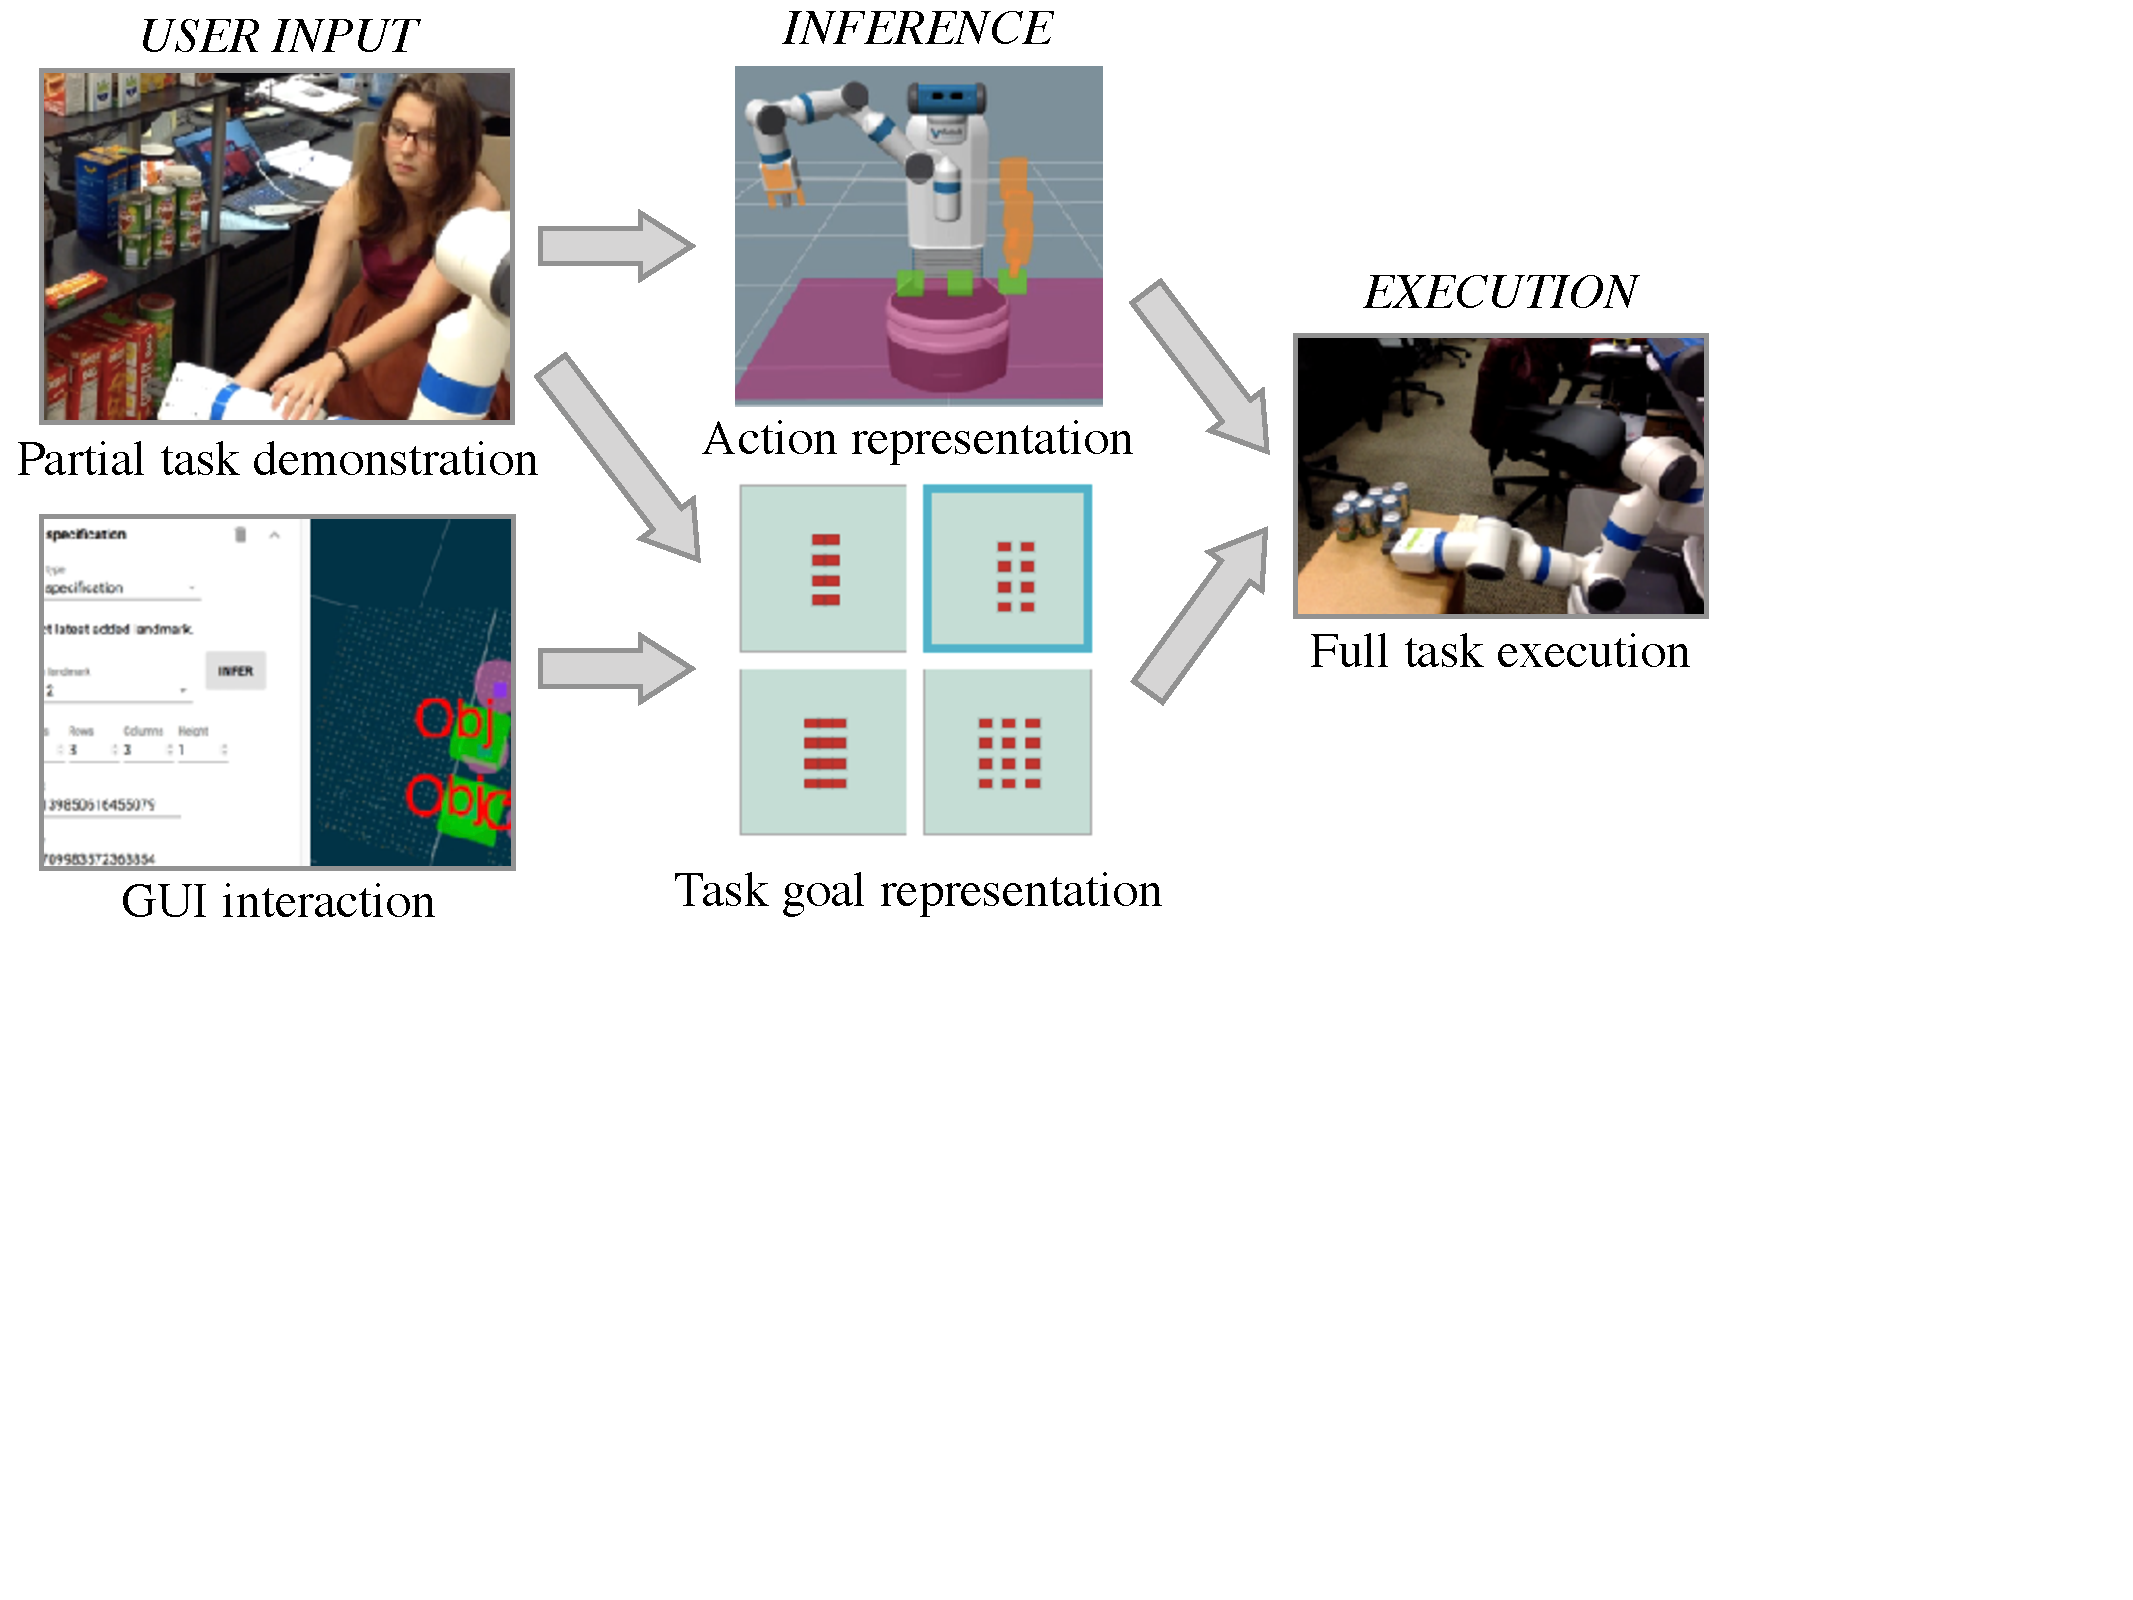
\includegraphics[width=0.85\linewidth]{figures/iros-overview}
	\caption{Overview of the developed system that allows users to demonstrate part of a shelf arrangement task and interact with a GUI to simultaneously program both the complete task goal (fully specified shelf arrangement) and the actions for achieving that goal.}
	\label{fig:irosoverview}
\end{figure}


In this chapter we propose an approach for enabling users to simultaneously program robotic shelf arrangement task goals and actions for a given item, by demonstrating a few steps of the shelf stocking task (\fig{fig:irosoverview}). 
We develop a user interface to visualise inferred task goals and actions, as well as enable other user input to augment their demonstrations. 
To better understand common structure in shelf arrangement tasks, we analysed the Freiburg dataset of close to 5,000 images covering more than 2,400 unique grocery items from 25 different categories (\cite{jund2016freiburg}). 
Our goal inference model, based on this dataset, takes demonstrations and other input from the user and proposes them most likely shelf arrangements in order to accelerate the teaching process.
We analyse how quickly correct goal configurations in the dataset can be inferred from user input according to 10 different teaching strategies.
We present an online user study that empirically investigates strategies that people use in a simplified arrangement task domain.
We implement our approach on a Fetch mobile manipulator and demonstrate the programming and execution of 8 arrangement tasks for objects from the dataset.

\subsection{Related work}
\label{sec:irosrelatedwork}

This work relates to several topics explored in previous robotics research.
The larger umbrella of end-user robot programming has seen a range of recent work focused on programming of mobile robots (\cite{huang2016design}), social robots (\cite{barakova2013end,glas2012interaction,glas2016human}), industrial manipulators (\cite{stenmark2017simplified}) and mobile manipulators (\cite{alexandrova2015roboflow,huang2017code3}).
The most widely explored approach is Programming by Demonstration (PbD) which involves taking demonstrations of a task as input and inferring the goal of the task or a policy that can be used to accomplish the task (\cite{billard2008robot,argall2009survey}).
A majority of the work focuses on directly learning a policy or modeling higher level actions from lower level control signals (\cite{schaal03,calinon09,akgun12klfd,schulmanlearning}), while some explore learning task goals or task structure represented in various ways (\cite{mohseni2015interactive,pardowitz2007incremental,ekvall2008robot,niekum2013incremental,jansen2006model}).
Most closely related to our approach, \cite{akgun2016simultaneously} explored simultaneous learning of actions and goals by demonstration, focusing on manipulation tasks, such as closing a box and pouring beans into a bowl.


%to teach a robot-specific manipulation task and a goal inference model to reduce the number of demonstrations required to learn the shelf arrangement task goal.
%Alexandrova et al. \cite{alexandrova2015roboflow} proposed a PbD system that involves preconditions and loops, but does not provide solutions for specifying  different configurations goal for shelf arrangement tasks.

Robot shelf stacking was part of the Amazon picking challenge in the last iteration (\cite{correll2016analysis}). 
Teaching robots to tidy up shelves was addressed previously by \cite{abdo2015robot}, but their focus is on dividing different products into categories, rather than configuring them on a shelf. 

%learns user preferences for tidying up shelves
%Our system learns the user preferences for shelf arrangement tasks, provides an interactive visualisation for the user to specify the configuration parameters and generalises the program to tasks with different products and configurations.
%Mees et al. learn spatial relations between objects such as on top, inside, next to using distance metric learning. https://arxiv.org/pdf/1703.01946.pdf
%Janson and Belpaeme, A model for inferring the intention in imitation tasks
%complex task structures (\eg \cite{,mohseni2015interactive}) 
%HTNs can be used to teach robots tasks by demonstration, but require `perfect' demonstrations,  are  generally assumed to be manually specified \cite{mohseni2015interactive}.
%pardowitz2007incremental

We argue for using end-user programming for teaching task goals and robot actions to perform arrangement of grocery items on shelves.
Shelf arrangements are different in every store; only the store owners or staff can correctly specify the task goals for the robot. 
Hence, the use of end-user programming is essential for that part of the problem. 
Previous work has explored alternative interfaces, such as speech or different GUIs for specifying task goals (\cite{alexandrova2015roboflow, kurenkov2015,nguyen2013ros}).
On the other hand, programming of actions is not necessarily tied to end-user programming.
An alternative is to give robots universal capabilities for grasping any object, planning a motion to move it without collisions, and placing it in any desired configuration. 
Motion plans could further involve non-prehensile actions (\cite{dogar2010push,king2015nonprehensile}) to reconfigure objects closer together as in some of the actions programmed by demonstration in this work. 
While a lot of research in robotics focuses on giving robots those capabilities, they are still far from being universal.
Another approach is for the robot to learn those actions by training on the job \ie self-exploration using reinforcement learning, but is likely undesirable due to long exploration times and negative impacts of trial errors.
%Organisation tasks can be automated in different ways: a domain expert can program the robot's joint positions to pick and place specific products but needs to reprogram these for new tasks and products
% use of planning approaches are commonly used but would still involve specifying grid configuration parameters (number of rows, columns, stacks, or object distances); pick and place actions can be automated using motion planning techniques but are prone to failures, especially for manipulations concerning varying object types and robot end-effectors (\eg non-prehensile approaches involving push-grasp actions \cite{dogar2010push,king2015nonprehensile}). 

\section{Approach}
\label{sec:irosorg-approach}

In this chapter we aim to enable a user to demonstrate part of the task of arranging an item on a shelf and have the robot complete the task on its own.
From the few user demonstrations, the robot needs to infer both {\em what} the desired arrangement of objects is and {\em how} to use its end effector to configure objects in the desired relative configuration. 
While both of these are well studied problems, their joint inference is common in previous work (\eg \cite{akgun2016simultaneously}). 
The specific challenge addressed in this chapter is the efficient inference of the task goal from few demonstrations that convey both goal and action. 
To that end, we explore two practical ideas:
\begin{enumerate}
	\item We perform a thorough analysis of the task domain to come up with compact domain-specific task representations that exploit common structure.
	\item We augment the user's input with direct specification of certain task parameters that are less efficiently conveyed through demonstrations. 
\end{enumerate}

We detail this approach in the following subsections.

\subsection{Freiburg Dataset Analysis}
\label{sec:irosdata-analysis}

The Freiburg dataset (\cite{jund2016freiburg}) contains 4,947 images of common grocery items and was originally collected for training visual classifiers.
We labeled the images according to product type and shelf arrangement. For the shelf arrangement data we excluded 998 (20.2\%) images that either did not show a supermarket shelf (\eg product on the table or vending machine) or that were duplicate images of a product on a shelf already included.
The remaining $3,949$ were used for understanding the structure of shelf arrangement tasks and defining a common task representation (\sect{sec:irosrepresentation}).

Our first observation is that almost all items in stores are arranged on a 2D or 3D {\em grid}.
We considered \textit{rows} to be the depth (front-to-back), \textit{columns} the width (left-to-right), and \textit{stacks} to be the height (bottom-to-top) of the grid.
As the dataset focused more on product types rather than product configuration, the configuration parameters were sometimes not all clearly identifiable.
The number of rows was often not visible but likely to be filled for the entire depth of the shelf.
Thus, we coded the specific number of columns and stacks and assumed rows to be \textit{as many as possible}.
%MC: The following sentence is not clear. 
% We labeled the data according to columns and stacks, and separately labeled those which were clearly identifiable.

Product packaging is often designed with the objective of compact packaging and efficient use of shelf space in stores.
As a result a large portion of items (54.3\% in our dataset) have a flat top surface that allow {\em stacking}, of which 33.9\% are rectangular prisms (\ie boxes) and 20.4\% are cylinders (\ie cans). 
Non-stackable items also have rectangular or circular bases to stand stably on the shelf surface, but less regular tops (\eg bottle lids) that prevent stable stacking (\fig{fig:types}).
We consider these objects equivalent to square pyramids (19.5\%) and cones (16.3\%).
Only 9\% of the items did not fit into the shape categories mentioned above and were categorised as soft packaging (8.7\%) or other (1.3\%), \eg triangular pyramid or hexagon prism.
\tbl{table:typesdistribution} shows the full distribution of the dataset across the categories of product types.

\begin{figure}[h]
	\centering      
	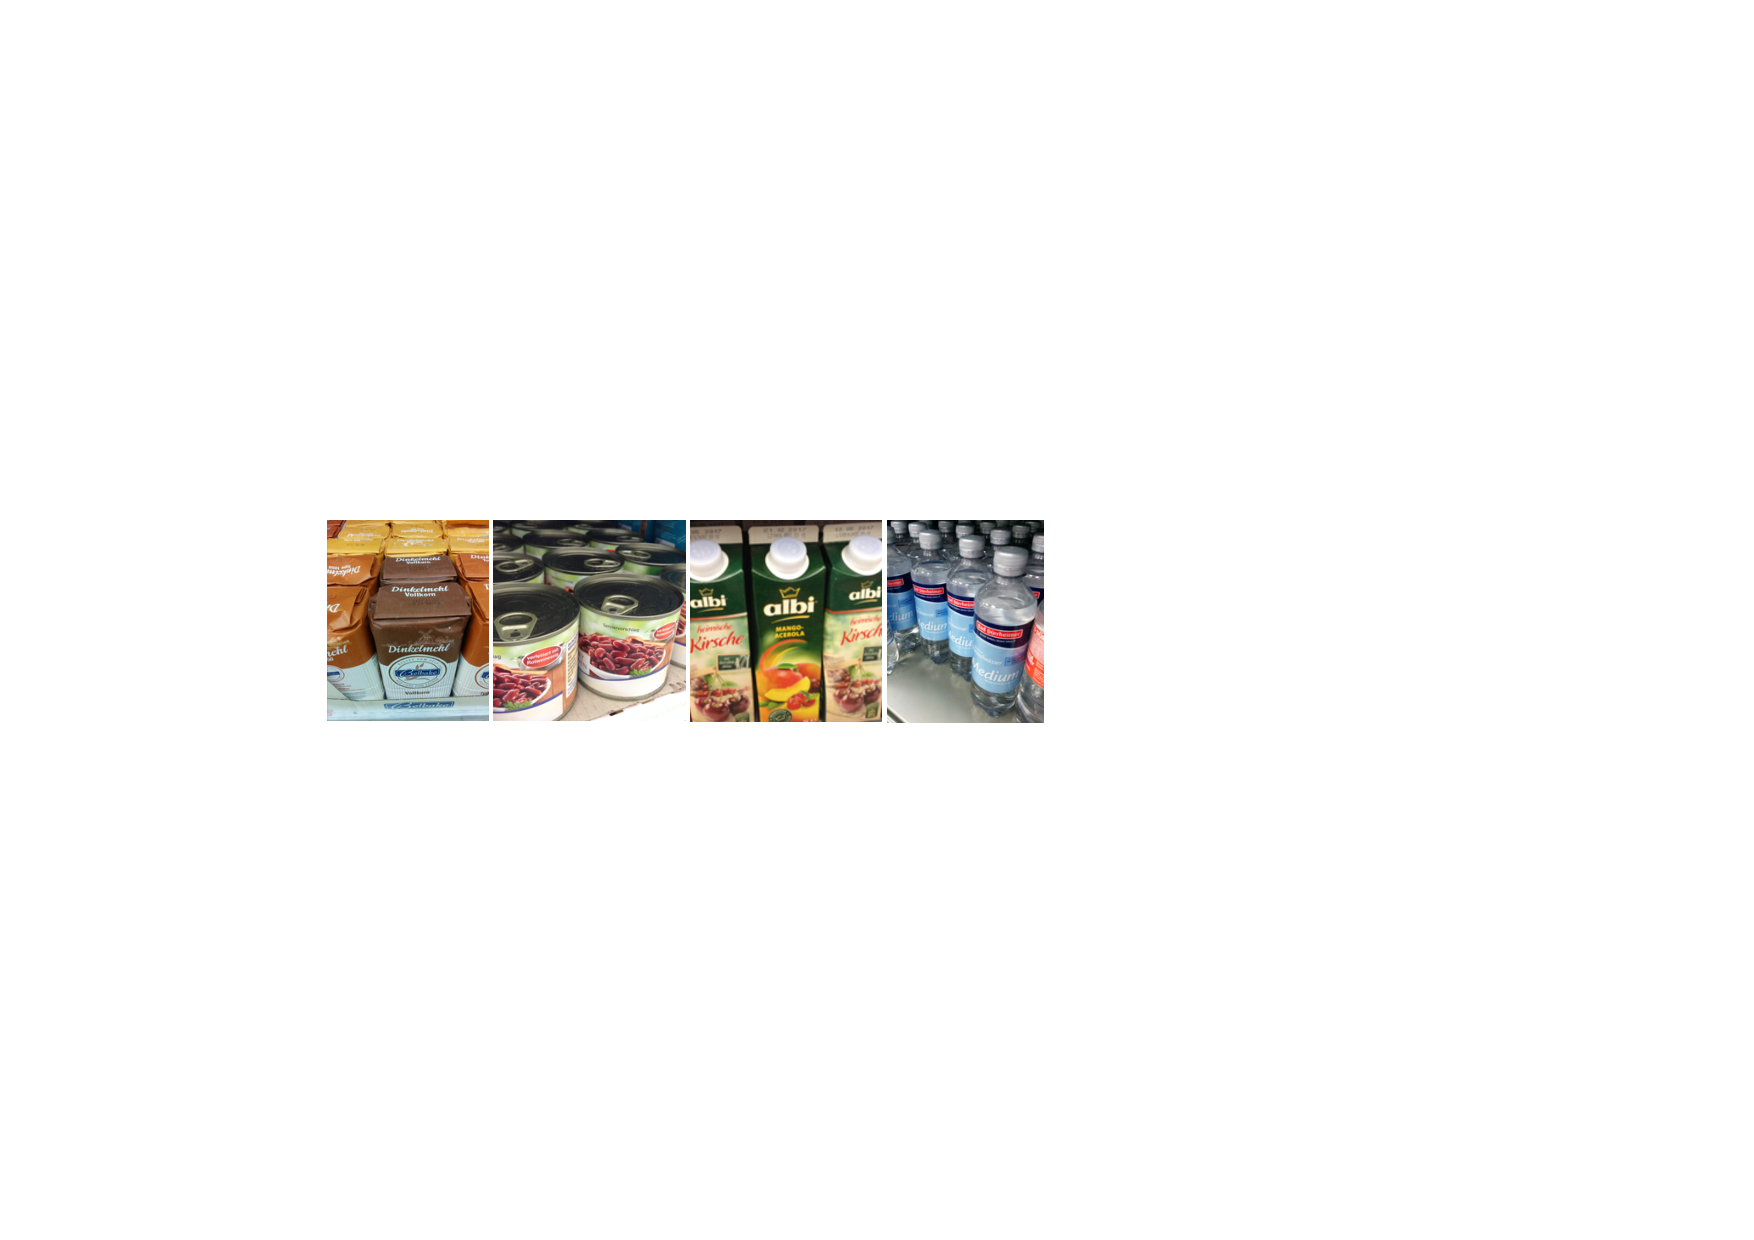
\includegraphics[width=0.6\linewidth]{figures/typespictures}
	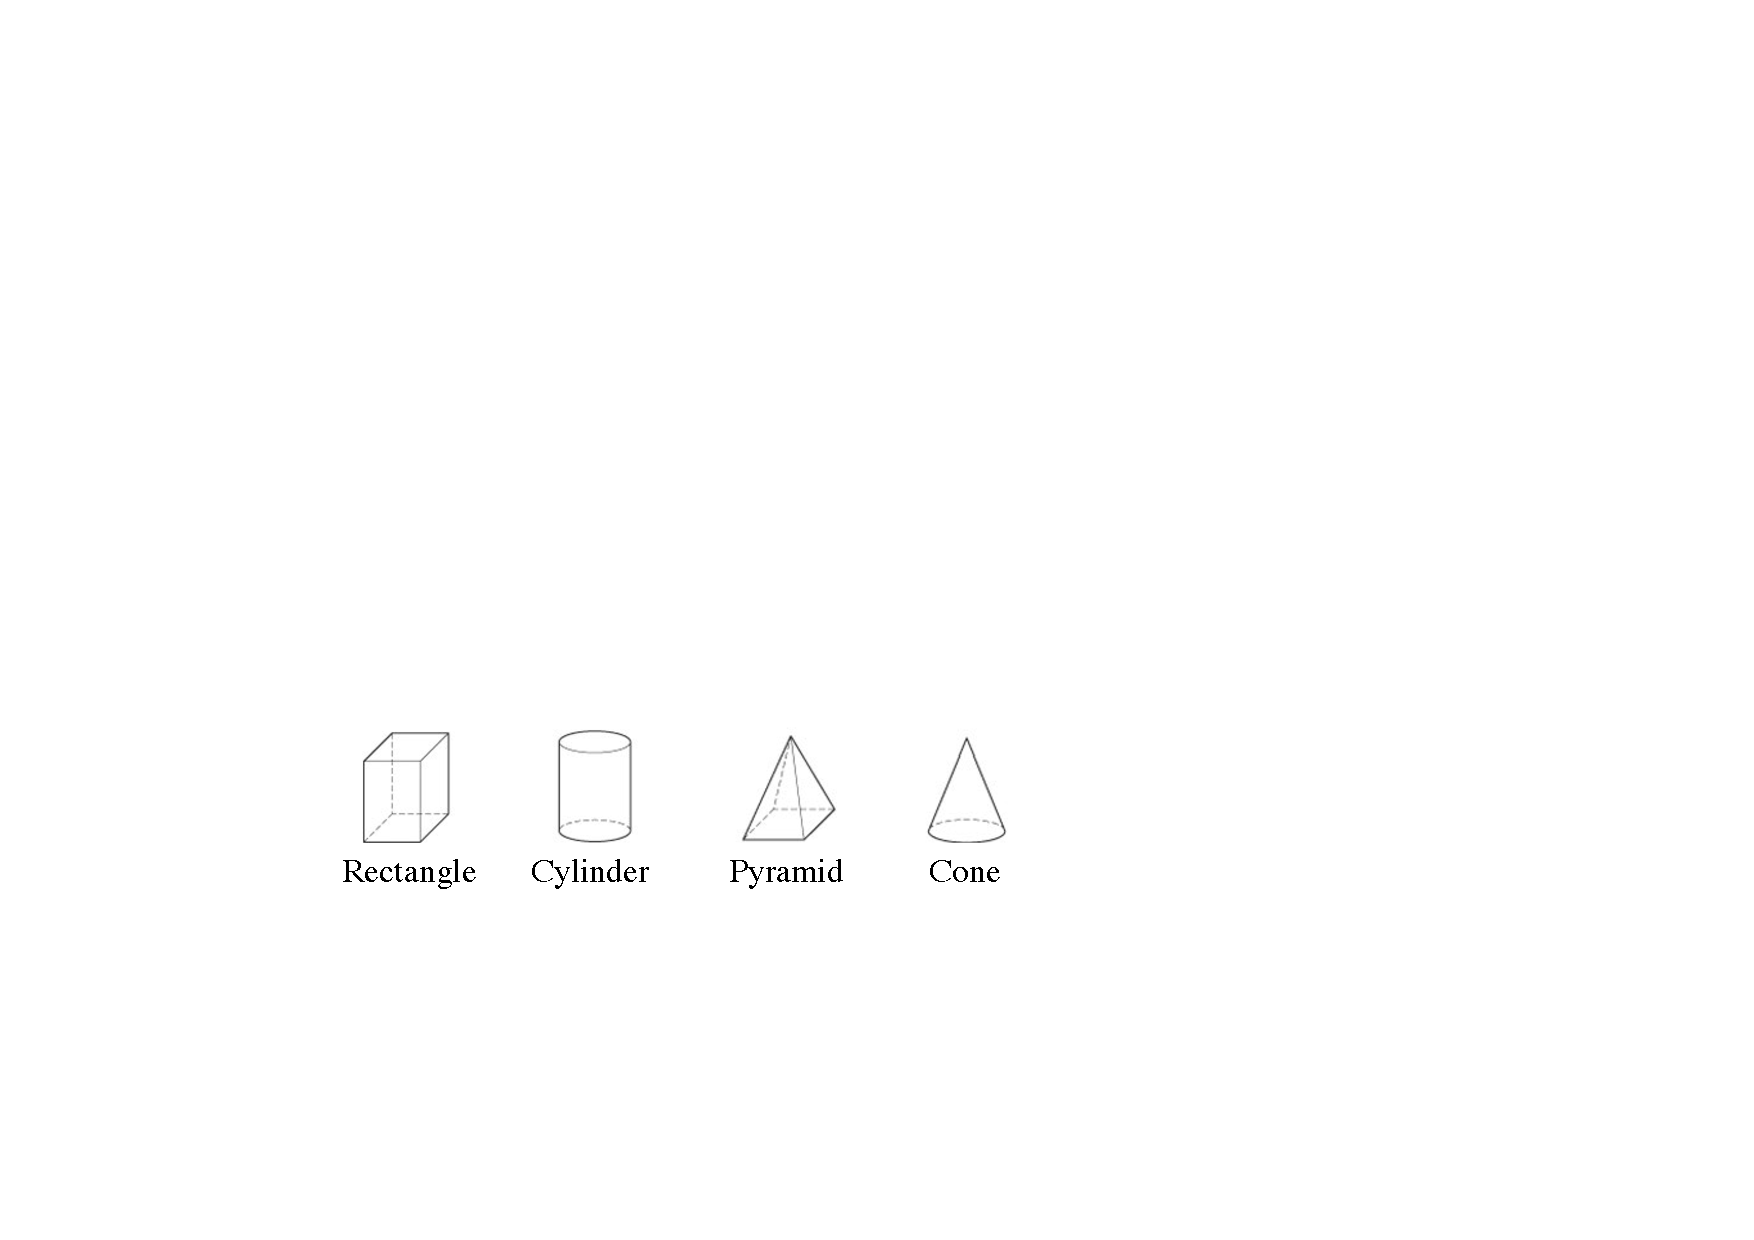
\includegraphics[width=0.6\linewidth]{figures/types}
	\caption{Main product shape categories, that comprise 90.1\% of items in the dataset, are defined based on the the shape of their base and their tip. The shape of the tip determines whether the objects can be stacked or not. The shape of the base determines whether the object is more compactly arranged on a regular grid (rectangular) or an off-grid arrangement (circular).}
	\label{fig:types}
\end{figure}


% MC: This is not needed as it is now spread across the text.
\begin{table}[h]
	\centering
	\caption{Distribution of product types found in the Freiburg dataset.}
	\label{table:typesdistribution}
	\begin{tabular}{r|cc}
		Product type category&Count& \% \\ \hline
		Rectangle (stackable, on-grid) &1676&33.9\% \\
		Cylinder (stackable, off-grid) &1011&20.4\% \\
		Square pyramid (not stackable, on-grid) &964&19.5\% \\
		Cone (not stackable, off-grid)&804&16.3\% \\
		Soft packaging: \eg candy &428&8.7\% \\
		Other: \eg triangular pyramid, hexagon prism &64&1.3\% \\ \hline
		Total &4947&100\%
	\end{tabular}
\end{table}

We also observe that items with rectangular bases are most compactly arranged on a grid with both side surfaces touching the neighbouring items (\fig{fig:off-grid}a).
Whereas objects with circular bases can be more tightly arranged when two consecutive rows are offset by half the radius length of the item, which we refer to as an {\em off-grid} arrangement (\fig{fig:off-grid}b).
Despite the compactness advantage, only a small percentage (1.75\%) of the dataset included off-grid configurations.
Although a majority of items were observed to be arranged as compactly as possible (touching neighbouring items on all sides), some arrangements left space between objects, possibly to allow customers to take items without knocking down others.
We observed that at least 0.26\% of arrangements left space between items either on the row or column direction (not possible in the stacking direction due to gravity).

\begin{figure}[h]
	\centering
	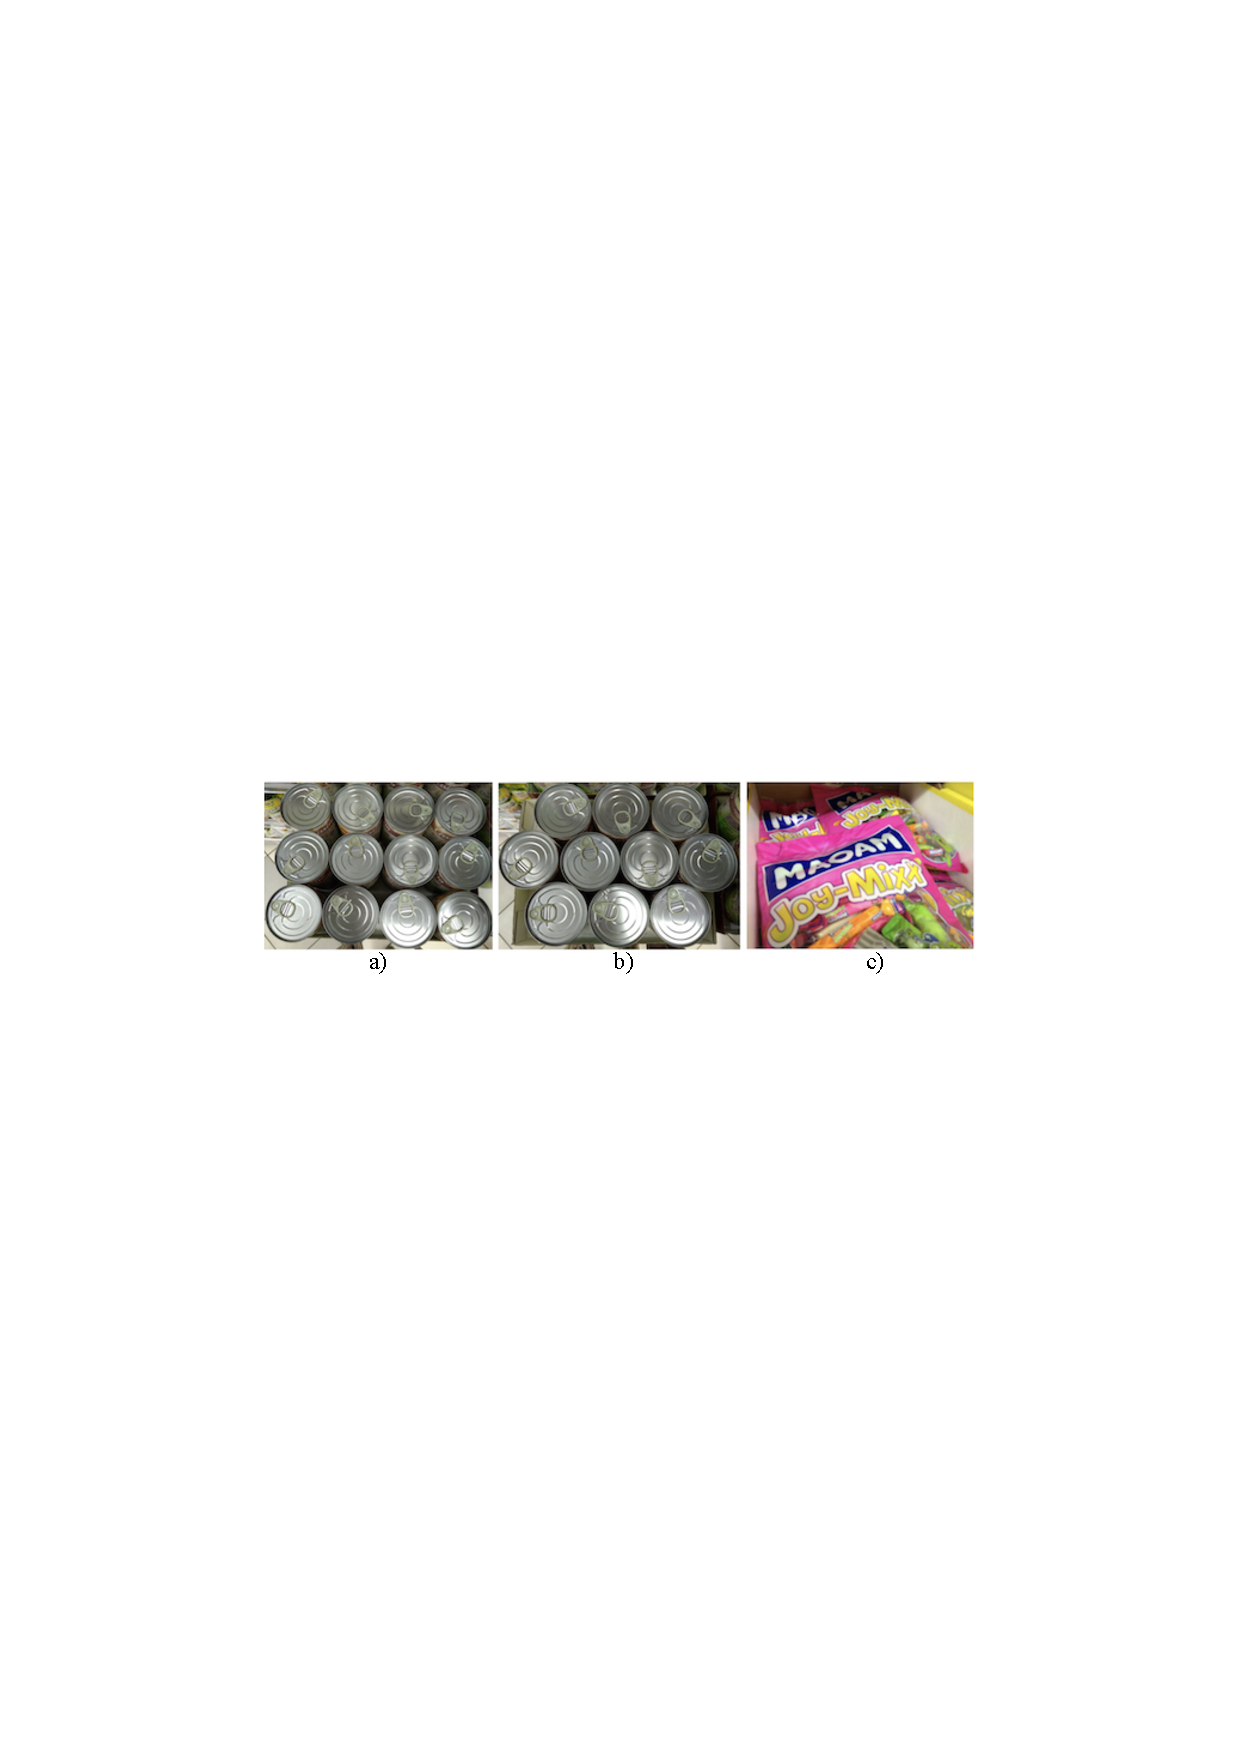
\includegraphics[width=0.8\linewidth]{figures/complex-config}
	\caption{Cylindrical item arranged in a) regular 3x4 grid and b) off-grid configurations. c) Soft-packaged item arranged in interleaved grid configuration.}
	\label{fig:off-grid}
\end{figure}



%We defined the following types to cover the products in the dataset (\fig{fig:types}): rectangle, cylinder, square pyramid, cone.
%The majority (90.1\%) of the products in the dataset can be categorised based on whether they are stackable (i.e. prism-shaped) or whether an off-grid configuration would save space (i.e. having a rectangular vs. circular base).


\subsection{Shelf Arrangement Representation}
\label{sec:irosrepresentation}

Based on the common product arrangements observed in the dataset, we propose a simplified grid-based task representation with the following variables: number of columns ($m$), rows ($n$), stacks ($s$), row distance ($d^n$) and column distance ($d^m$), where $m, n, s \geq 1$ and $d^m, d^n \in \{0,1\}$ represent the binary state for touching and not touching respectively.
Thus, we represent a shelf arrangement task (where the shelf is orthogonal to the robot) as a tuple $\tau = (n, m, s,d^n,d^m)$. 
\tbl{tab:data-analysis} shows the distribution of the values for these variables observed in the Freiburg dataset.
Note that this representation excludes soft-packaged or irregularly shaped items, as well as off-grid arrangements.
However, the representation could easily be extended for more complex tasks, such as continuous values for $d^n$ and $d^m$, variables describing off-grid configurations, or variables for orientation of the items.

\begin{table}[h]
	\centering
	\caption{The distribution of shelf arrangement parameter values across the Freiburg dataset.}
	\label{tab:data-analysis}
	\begin{tabular}{r|rrrrrrr}
		\multicolumn{1}{l}{} & \multicolumn{5}{c}{stacks} & \multicolumn{1}{l}{} \\
		columns & \multicolumn{1}{c}{1} & \multicolumn{1}{c}{2} & \multicolumn{1}{c}{3} & \multicolumn{1}{c}{4} & \multicolumn{1}{c}{\textgreater4} & \multicolumn{1}{l}{\textbf{}} \\ \hline
		1 & 49.4\% & 4.4\% & 0.7\% & 0.2\% & 2.3\% & \textbf{57\%} \\
		2 & 29.6\% & 3.4\% & 0.4\% & 0\% & 1.4\% & \textbf{35\%} \\
		3 & 5.8\% & 0.5\% & 0\% & 0\% & 0\% & \textbf{6\%} \\
		4 & 1.3\% & 0.2\% & 0\% & 0\% & 0.1\% & \textbf{2\%} \\
		5 & 0.1\% & 0\% & 0\% & 0\% & 0\% & \textbf{0\%} \\
		6 & 0\% & 0\% & 0\% & 0\% & 0\% & \textbf{0\%} \\
		7 & 0\% & 0\% & 0\% & 0\% & 0\% & \textbf{0\%} \\
		& \textbf{86\%} & \textbf{8\%} & \textbf{1\%} & \textbf{0\%} & \textbf{4\%} & \textbf{100\%}
	\end{tabular}
\end{table}
% generated using https://www.tablesgenerator.com/latex_tables#

% \begin{figure}
% 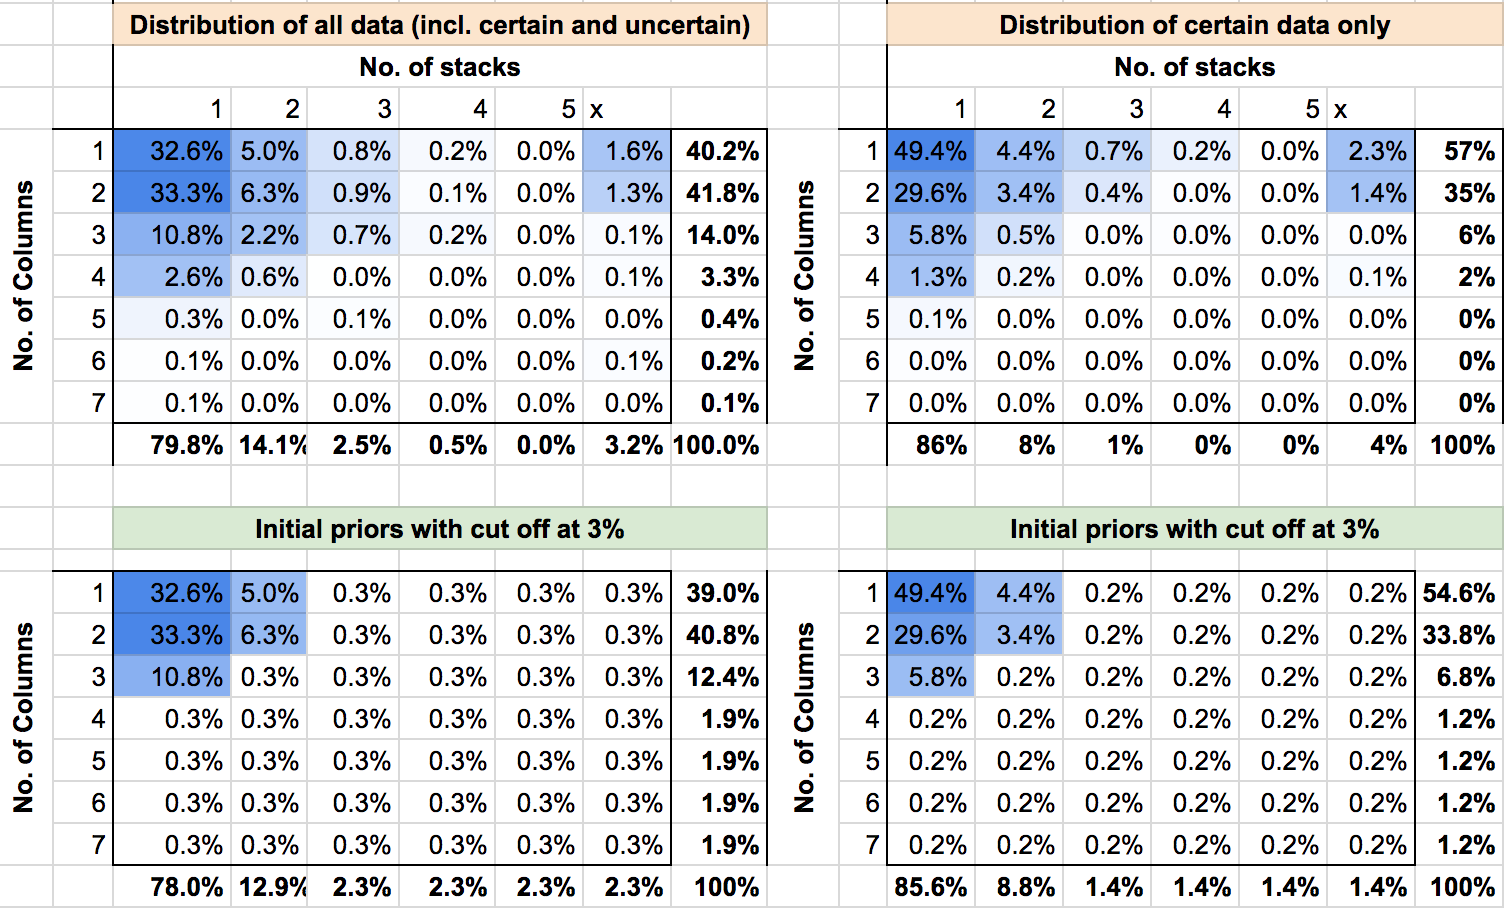
\includegraphics[width=\linewidth]{figures/data-analysis}
% \caption{Freiburg dataset analysis (of 3,949 images) for observed number of columns and stacks (top) and derived priors for goal inference model (bottom): all data (left) vs. certain data only (right) \todo{Convert this into a regular latex table showing only certain frequencies (no need for uncertain and priors).} }
% \label{fig:data-analysis}
% \end{figure}


\subsection{Goal Inference from Demonstration}
\label{sec:irosinference}

%For each possible configuration $\tau_i = (n_i,m_i,s_i,dn_i,dm_i)$, 
%by ranking all possible configurations.
The problem of goal inference is the estimation of most likely shelf arrangement based on the input obtained from the user.
We represent this as a maximum a posteriori estimation problem, \ie
\begin{equation} \label{eqn:optimize}
\tau^* = \underset{\tau_i \in T}{\arg\max} P(\tau_i|D)
\end{equation}
where $T$ is the set of all possible shelf configurations and $D = \{ A_j, O_j \}_{j=1}^{M}$ is the set of $M$ demonstrations provided by the user with $A_j$ actions each leading to the placement of one additional object on the shelf. 
Hence, each $O_j$ corresponds to configurations $(x, y, \theta, s) \in (\mathbb{SE}2 \times \mathbb{N})$ ($s$ for stack number) of $j$ objects that have been placed so far on the shelf surface or on top of another object.
%Given a sequence of demonstrations $D = D_1, D_2, ...$, where $D_i = (n_i,m_i,s_i,dn_i,dm_i)$ represents a configuration similar to the goal configuration $\tau_G$, 
Since the demonstrations are assumed to be progressions of the same shelf configuration task, the goal inference only depends on the latest shelf configuration $O_M$ rather than all of $D$.

Given the $M$ object configurations in $O_M$ we estimate the current shelf arrangement $\tau_M = (n_M, m_M, s_M, d^n_M, d^m_M)$ as follows. 
The number of rows and columns are determined by separately finding alignments (\ie values within a small distance) in $x$ and $y$ dimensions of the objects.
The number of aligned groups gives the number of estimated rows and columns ($n_M, m_M$).
The number of stacks ($s_M$) is estimated as the highest stack number of any object in the demonstrated configuration.
The contact between rows and columns  ($d^n_M, d^m_M$) are estimated based on the majority relation between rows and columns.

Next, we substitute $\tau_M$ for $D$ and use the Bayes Rule to calculate the posteriors of the term we would like to maximise as follows:
$$P(\tau_i|\tau_M) = \frac{P(\tau_M|\tau_i)P(\tau_i)}{\underset{\tau_j \in T}{\sum} P(\tau_M|\tau_j)P(\tau_j)}$$

We assume that the probability $P(\tau_M | \tau_i)$ is zero for all $\tau_i$ whose row, column, and stack parameter values are already exceeded in $\tau_M$.
Similarly, any arrangement $\tau_i$ whose binary variable ($d^n, d^m$) is contradicted in the demonstration is considered zero.
%For example, if inferred shelf arrangement from the latest configuration $O_M$ is $\tau_M = (3,4,1,0,0)$, then $P(\tau_M | (3,3,1,0,0))=0$ whereas $P(\tau_M | (3,5,1,0,0))>0$.
Note that $d^n$ and $d^m$ are only relevant if there are at least two rows or columns respectively ($n$$>$1, $m$$>$1).
We initialise the priors $P(\tau_i)$ based on their observed occurrence in the dataset (\sect{sec:irosdata-analysis}).
To have a finite set of possible shelf configurations we bound the grid parameters based on the dataset as well, where $m \in [1..7]$, $n \in [1..2]$ and $s \in [1..5]$, where $n=2$ corresponds to having \textit{as many rows as possible} based on the shelf, rather than an exact number of rows.

%(\ie $n_D > n_i, m_D > m_i, s_D > s_i$), or if $dn_D \neq dn_i$ or $dm_D \neq dm_i$. 
%We are interested in the probability $P(\tau_i)$ that $\tau_i$ is the \textit{ground truth} $\tau_G$, i.e. the user's desired goal configuration. 

%XXXX Going from max to ranking XXX
While the computation in Equation \ref{eqn:optimize} gives a single most likely configuration, we propose to give the top few arrangements with the highest likelihoods as {\em suggestions} to the user.
This requires ranking all possible arrangements in terms of their likelihoods, given the demonstration.
Since ties are possible due to equal priors we rank configurations with smaller parameter values as higher.

\subsection{Goal Inference with Direct Specification}
\label{sec:irosspecification}

To allow the user to directly specify goal shelf arrangement parameters to augment demonstrations, we exploit the way that our goal inference works as described in Section \ref{sec:irosinference}.
If the user directly specifies the value of a goal arrangement parameter, all arrangements that are inconsistent with that specification are considered to have zero probability. 
This corresponds to a slight change in the formulation, where the input from the user relevant for the inference does not only include $\tau_M$ but also any direct specification $\mathcal{S}$, where $P(\tau_i | \mathcal{S}, \tau_M)$ is zero if $\tau_i$ is inconsistent with $\mathcal{S}$.
This allows for a fast elimination of many candidate arrangements.


\subsection{Action Representation and Inference}
\label{sec:irosactions}

We use a simple action representation proposed in previous work (\cite{akgun2012keyframe,alexandrova2014robot}).
We assume that the robot can perceive the configuration of the shelf and of each object on it.
Each of these perceived entities are considered as potential {\em landmarks}.
The action is then represented as a sparse sequence of end-effector poses relative to one of the landmarks and gripper states (open/close).
For example, placement of an object next to another object could be done by moving the gripper to a pose near the reference object, lower the gripper, open the gripper, clear the gripper from potential collisions. All of these poses would be relative to the reference object. Non-prehensile actions, such as moving the placed object closer to the reference object, could also be easily represented in the same way, as poses of the gripper relative to detected objects.

Such actions can be directly programmed with a single demonstration using heuristic assignment of poses to landmarks.
The assignment can then be corrected by the user (\cite{alexandrova2014robot}) or through multiple demonstrations of the same step (\cite{niekum2012learning}).
We take the first approach; hence an individual action demonstration in $A_j$ is already an executable action.
%Our system differs from \cite{alexandrova2014robot} as it allows the user to specify exact pose coordinates on the user-interface which gives the user more control over the learned action.
While there can be ways to combine multiple demonstrations, in our implementation the robot randomly chooses an action from the subset of $A_j$ that is reachable based on the configuration of landmarks in the scene.
Although all demonstrated actions should be reachable for the objects in the shelf arrangement that were placed during the demonstration, some actions may become unreachable when they are shifted for placement of other objects to complete the desired shelf arrangement.
Hence having multiple demonstrations in $A_j$ is still valuable.

Execution of actions simply involved detecting all landmarks in the environment, computing the actual configuration of end-effector poses that are relative to those landmarks, and then moving through the landmarks one by one.

\subsection{Implementation}
\label{sec:irosimplementation}
%\subsection{Keyframe-based Programming by Demonstration}

We implemented our approach on a Fetch mobile manipulator which has a 7-DoF arm with a load capacity of 6kg.
Our system builds on the open-source system Rapid PbD (\cite{rapidpbd}) which implements the action representation described in Section \ref{sec:irosactions}.
The robot detects the shelf surface and objects on it using standard Point Cloud Library functionality.
As stacked objects are perceived as one cluster on the surface, we detect stacking from height changes that are approximately equivalent to the height of the object measured at the demonstration of the first action.

We extend the Rapid PbD graphical user interface (GUI) in several ways.
Users first create an empty program using the GUI.
Then they kinesthetically move the robot arm to desired poses and save poses or change the gripper state through the GUI.
We assume that the items to be placed on the shelf are always picked up from the same location.
Demonstrations involve a sequence of picking, moving, placing, and possibly non-prehensile readjusting of one object relative to the shelf or to another object already on the shelf.

When the user confirms the end of an action demonstration the robot perceives the end state of the demonstration $O_M$, which is expected to include $M$ objects.
The robot then infers $\tau_M$ as described in Section \ref{sec:irosinference} and visualises the most likely configuration overlaid onto the detected objects that are already placed (\fig{fig:gui}).
In our implementation the average row and column distances ($d^m, d^n \geq 0$) are read from the demonstrated arrangement and off-grid arrangements are recognised.
The user can create interleaved arrangements (\fig{fig:off-grid}c) by changing $d^m, d^n$ on the GUI.
It also displays the top four arrangements that have the highest likelihood given the demonstrations so far.
The GUI allows the user to select an arrangement from this list or directly specify task goal parameters (\sect{sec:irosspecification}).
When the goal for the shelf arrangement is confirmed, the robot can execute the complete shelf arrangement task either continuing from what has already been demonstrated or starting from scratch.


%On program execution, the robot goes through the steps and moves its end-effector to the poses relative to the landmarks on the table.
% which represents a program as a sequence of steps consisting of actions to command the robot's end-effector poses, gripper status, head movement or table top detection.
% The system uses keyframe-based PbD \cite{akgun2012keyframe}, where demonstrations are provided by kinesthetically manipulating the robot's arm and recording a series of end-effector positions (or \textit{keyframes}). 
% An end-effector pose can be relative to the robot's base or to a landmark previously detected by the robot.
% Landmarks are only known to the robot after a table top detection step has been performed.

% MC: Does not add too much but we can remove if needed.
\begin{figure}
	\begin{center}
		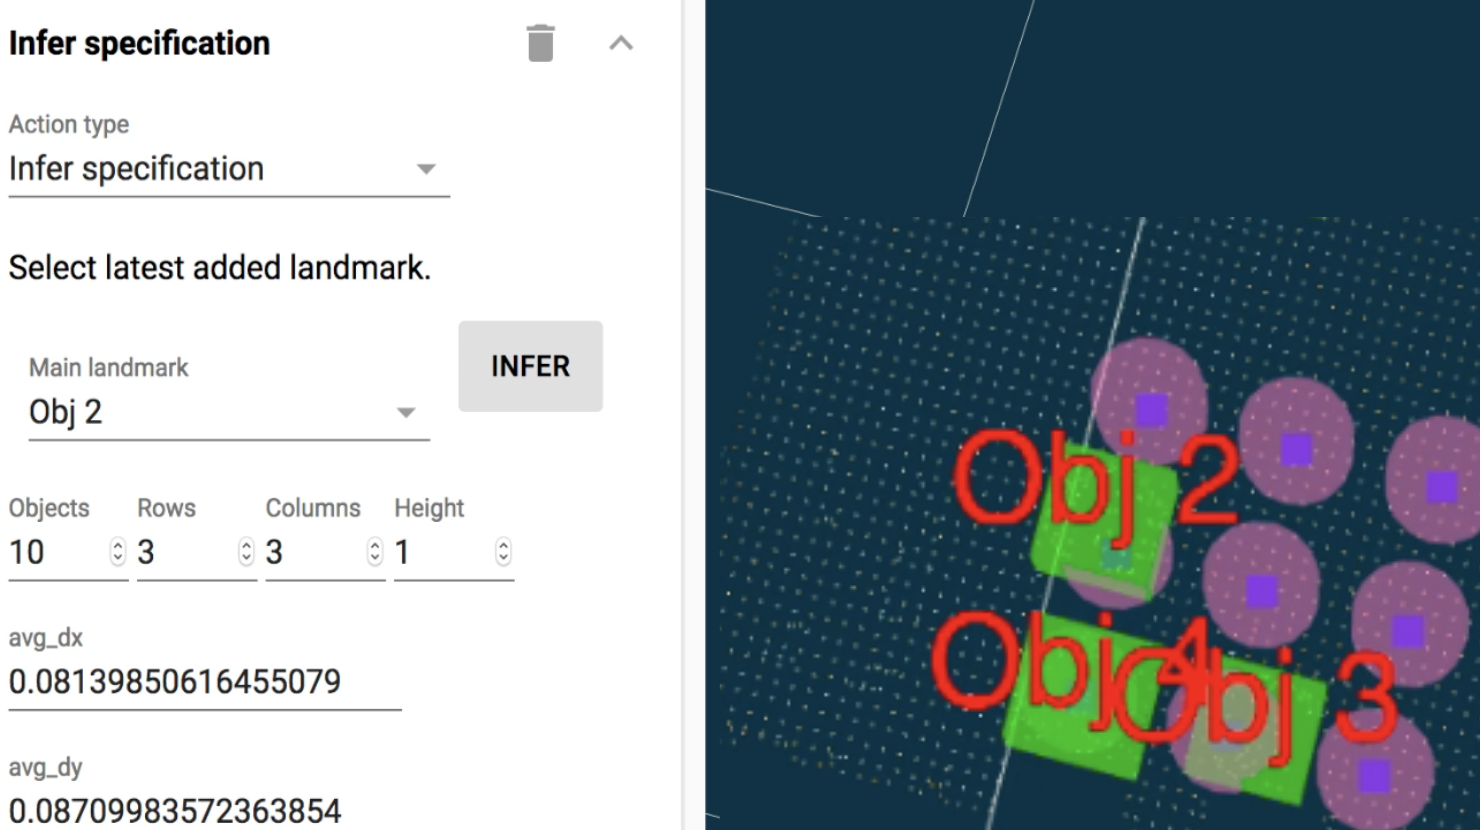
\includegraphics[width=0.8\linewidth]{figures/gui-iros}
		\caption{The extended Rapid PbD interface with the inferred object arrangement (purple) visualised overlaying the detected objects (green).}
		\label{fig:gui}
	\end{center}
\end{figure}


%\subsection{PbD for Shelf Organisation}
%As mentioned previously, we address grid-shaped shelf stocking tasks which generally involve arranging multiple objects of the same type.
%To program a task, the user first needs to create a program of a single pick and place action and use the table top detection step to register the object's dimension and position.
%Our system uses this information to infer grid configuration parameters and the task goal, which can be visualised on the graphical interface .
%It is assumed that the first object is on the top right corner (from the robot's perspective) and uses the inferred parameters to populate the grid positions.

% MC: This is inconsistent with the binary dn dm described in the approach section.
%Row and column distances ($dn$ and $dm$) have continuous values and set to the average distance in the demonstrated configuration.
%The user can provide input in the form of demonstrations, parameter specification (number of rows, columns, stacks, objects, row or column distance), or by selecting a suggested likely configuration. 
%After a new demonstration, the system perceives the configuration and updates the ranking of the most likely arrangements using the goal inference model. 
%On program execution, the robot computes the end-effector poses for each grid position and performs the demonstrated pick and place action consecutively. To ensure a successful execution of the final task, the user can run the program for a subset of objects as part of the programming process. 

%\subsection{Reusable Programs}
%\label{sec:irosresuableprogram}

Our interface also allows users to reuse previously programmed tasks and actions for shelf arrangement with different objects or grid parameters.
To that end the user can set up full or partial shelf arrangements and then run the object detection and goal inference.
They can also change task parameters to match the new task.
Programmed manipulation actions can also be transferred in some cases, but need to be tested and possibly adjusted to work with different objects.

%We enable the user to modify the program in order to reuse the taught manipulation action for arrangement tasks with different objects or grid parameters. The user simply needs to rerun the table top detection and the goal inference steps so that the system can register the new object's position and dimensions and recalculate the grid parameters. The user may need to test the task execution on a smaller subset of objects to ensure that the previously taught manipulation action is suitable for the new object. The grid parameters can be changed on the interface and the modified program can be executed for the new task. 

%%%%%%%%%%%%%%%%%%%%%%%%%%%%%%%%%%%%%%

\section{Goal Inference Evaluation}\label{sec:irosinfeval}
We evaluate our approach in three ways.
First, in this section we present (1) a systematic evaluation of the goal inference on the Freiburg dataset and (2) a user evaluation through an online study with a simplified interface. Next, in Section \ref{sec:irossystemeval} we present the full system evaluation.

%goal inference model by conducting a user study with 32 participants on Amazon Mechanical Turk (AMT). First, we initialised our goal inference model with priors based on our large-scale dataset (\fig{fig:data-analysis}). Then, we defined teacher actions and teaching strategies and simulated their performance for the use cases observed in the dataset. Finally, we conducted user studies on AMT and observed the usability of our model, as well as the user's preferred teaching strategies. 

\subsection{Teaching Strategies}
\label{sec:irosstrategies}

Our system provides the user with different possibilities for programming shelf arrangement tasks. 
As described in Section \ref{sec:irosinference}, at any point during the programming process the user has three possible actions:
\begin{itemize}
	\item \textit{Demonstrate} object placement kinesthetically, % ($2c$)
	\item \textit{Specify} grid parameters on the interface, % ($c$)
	\item \textit{Select} an arrangement from most likely arrangements, % ($c \times \frac{p}{N}$)
\end{itemize}
%% MC: The fraction cost for select does not make sense to me.
%where $c$ is a unit cost (\eg time to perform the action), $p$ is the number of likely arrangements proposed to the user and $N$ is the total number of arrangements.

The user can have different strategies for using a combination of the different actions to minimise cost.
Often times, learning algorithms are evaluated with {\em sample efficiency}, \ie the number of examples needed to learn a concept.
Similarly, users of our system can try to minimise the number of programming actions they need to take in order to correctly teach a shelf arrangement.
Alternatively, each action can be associated with a different cost, such as {\em clock time} and the user can try to minimise that cost.

Given the three programming actions above, we devised the following programming strategies:
\begin{enumerate}
	\item Naive demonstration (ND) involves demonstrating the full shelf arrangement filling up rows, columns, and stacks in progression.
	\item Optimal demonstration (OD) involves giving the minimum number of demonstrations to make the inference correct; \ie filling up one row, one column and one stack.
	\item Demonstrate and specify (D\&S) involves demonstrating distances $d^m$ and $d^n$ and specifying remaining variables $n,m,s$.
	\item Naive specification (NS) involves specifying all values in order of $n, m, s, d^n, d^m$.
	\item Prior-aware specification (PaS) involves only specifying values that are different from the most likely values according to the prior.
\end{enumerate}

These programming strategies are akin to optimal teaching algorithms that can be devised for a given concept and known learner (\cite{cakmak2012aaai,khan2011humans}).
The selection action can be used in combination with any of these strategies, therefore resulting in 10 teaching strategies.
We assume that the interface displays the top four most likely configurations.
Hence if the most desired arrangement is in the top four, the user can directly select this configuration and complete the programming process.
Note that in order to learn the action as well as the task goal, the robot needs to obtain at least one demonstration from the user, which is not the case for all strategies.
However, for the purposes of the analysis of goal inference, we ignore that fact.
In practice, those strategies that do not involve any demonstrations would require at least one demonstration in addition to the other programming steps.

%(see Sec. \ref{sec:irosdata-analysis}). For the specify action, the fields were initialised to $(1,1,1,-1,-1)$ and a step was counted only if a value needed to be changed. The prior-aware strategy checks the likely arrangements proposed and first specifies the parameters which are different to the ones shown. 
%The cost associated with \textit{select} can be considered a cost to inspect the proposed arrangements, which increases with the number of proposals shown.



\subsection{Evaluation on the Freiburg Dataset}
We measured the performance of each teaching strategy in terms of the number of steps required to infer the desired arrangement across the Freiburg dataset.
Figure \ref{fig:rankVSsteps} shows the learning curves for the ten teaching strategies for four example shelf configurations.
We observe that for simpler configurations ($m,n,s \leq 2$), strategies that involve demonstrations are comparable or better than specification strategies, because (1) $d^n, d^m$ are automatically inferred from the object placements and (2) our priors are based on the dataset where simpler configurations are ranked higher.

For higher $m,n,s$ values, the na\"{\i}ve demonstrations become infeasible, optimal demonstrations are bounded by $(n+m+s-2)$ steps, while specification strategies are always bounded by a maximum of 5 steps. 
%Based on the simulations, we chose the number of likely arrangements to be proposed to the user as 4 and defined additional teaching strategies, which include directly selecting the desired arrangement from the proposals before it reaches the top rank. 
The version of each strategy that involves a final selection step from the top four arrangements is more efficient or the same (in terms of number of actions) as the original strategy, since it takes fewer demonstrations or specifications to get the desired arrangement in top four versus top one. 
The most efficient strategy is the \textit{prior-aware specify+select} strategy requiring 1.85 steps on average. 

Overall, the average number of steps required to teach shelf configurations for all teaching strategies (\fig{fig:avgSteps}) is low (between 2-3 actions) despite some outlier cases (\eg \textit{naive demonstrations} requiring over 50 demonstrations (\fig{fig:rankVSsteps})).
This is a positive outcome of using priors that are based on the dataset, which in turn allows faster inference on the majority of the data.

\begin{figure}[h]
	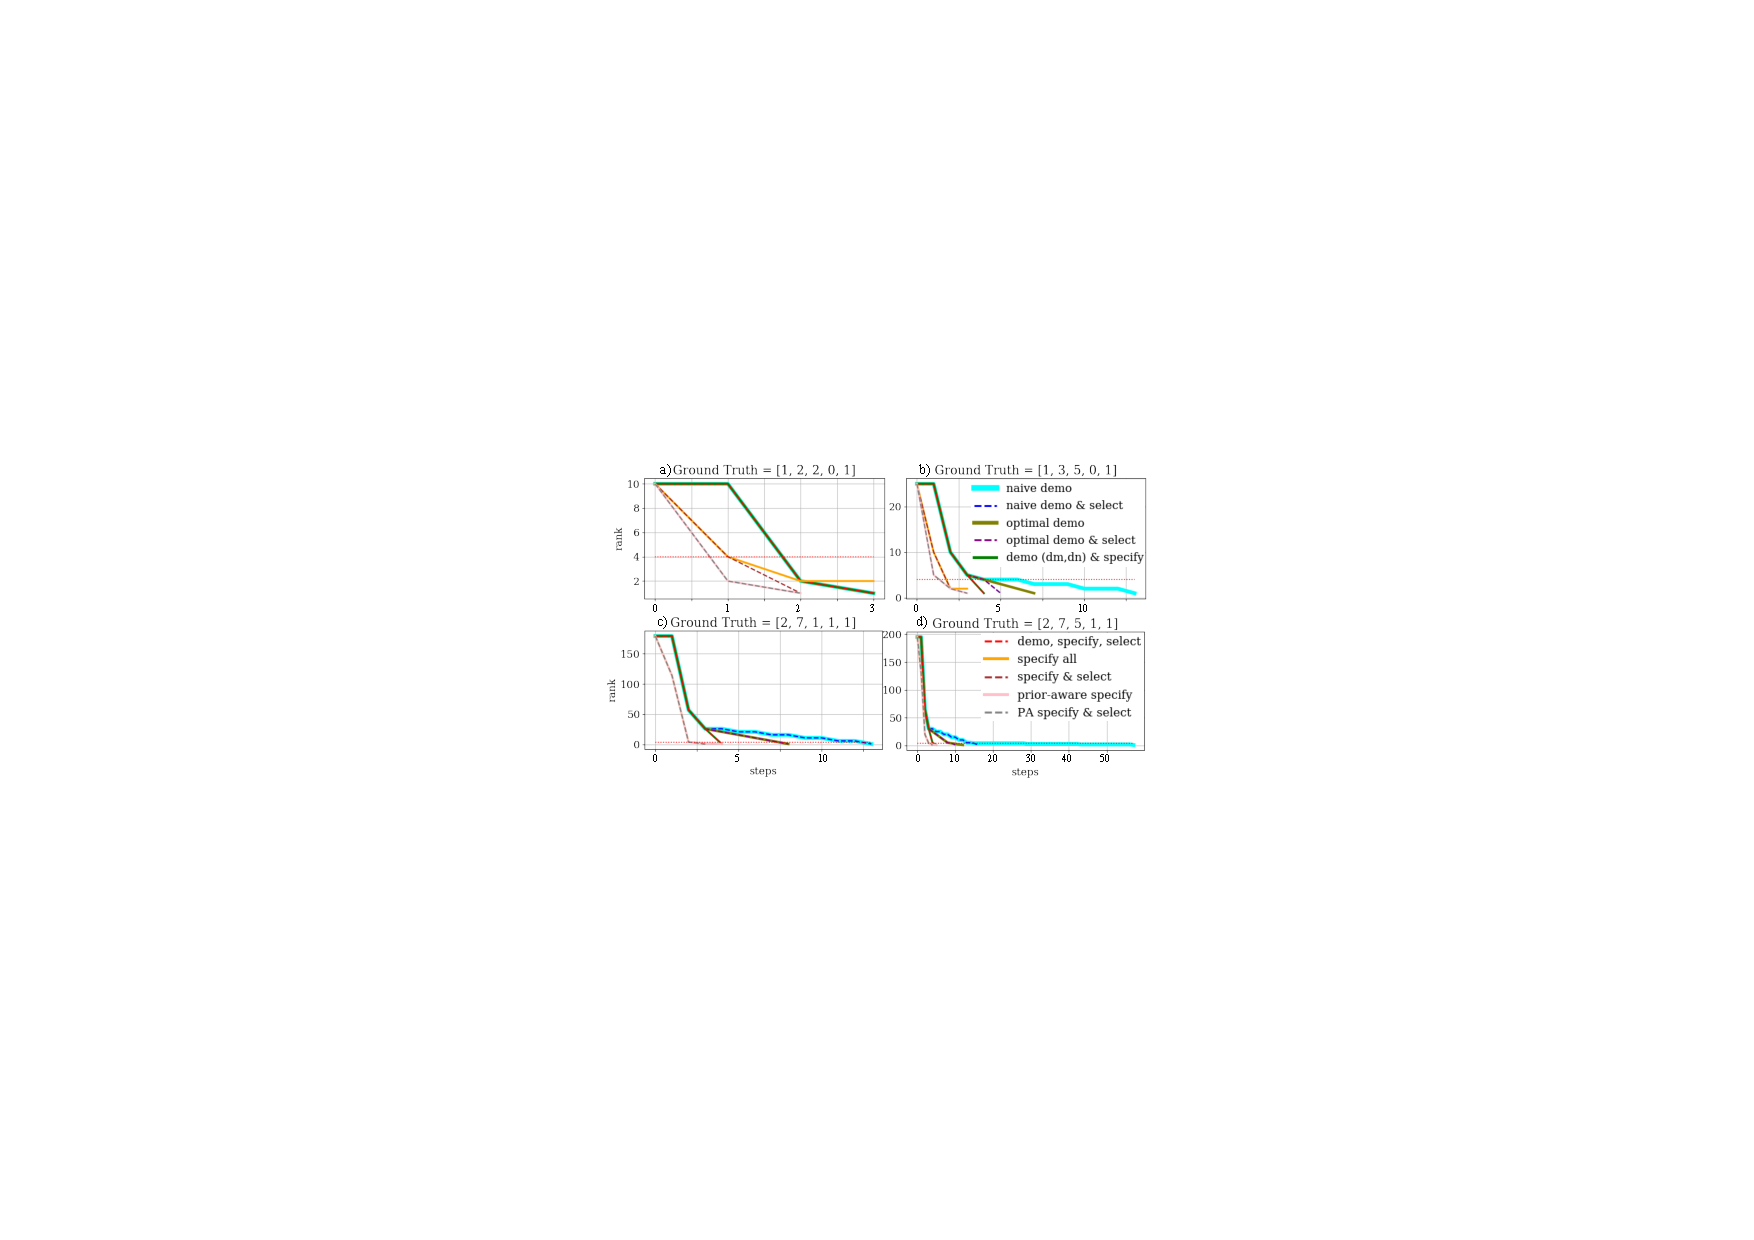
\includegraphics[width=\linewidth]{figures/rankVsSteps-new}
	\caption{Learning curve of 10 teaching strategies for 4 different shelf arrangements from the Freiburg dataset, with number of actions (x-axis) and ranking of the ground truth shelf arrangement (y-axis). For simpler configurations (a), demonstration strategies are comparable or better than specification strategies. For higher configurations, na\"{\i}ve demonstrations become infeasible (b-d).}
	\label{fig:rankVSsteps}
\end{figure}

\begin{figure}[h]
	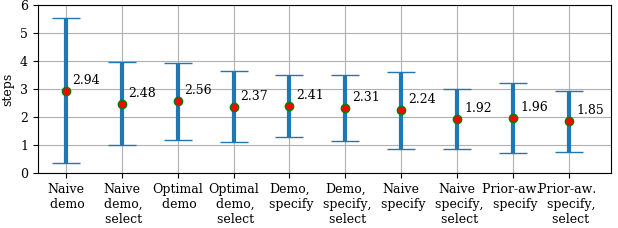
\includegraphics[width=\linewidth]{figures/avgSteps-certain-data}
	\caption{Average number of steps required to infer the correct arrangement per teaching strategy across the dataset (error bars show standard deviation).}
	\label{fig:avgSteps}
\end{figure}


\subsection{User Study Evaluation}
Next we conducted a user study on Amazon Mechanical Turk (AMT)\footnote{\url{www.requester.mturk.com}}, an online crowd-sourcing platform used to solicit and compensate participants for user studies (\cite{kittur2008crowdsourcing}).
%Mechanical Turk was found to be an appropriate platform based on free-form responses elicited from the workers in a pilot study. 
%The responses to the open-ended questions were also used for filtering the data obtained in experiments. Data from participants who did not provide any open-ended response, or whose responses were not comprehensible were removed and a new participant was recruited to replace it. 
%An individual was allowed to take part only once in any of our experiments.
The aim was to evaluate the goal inference method and investigate teaching strategies preferred by human users. 
For this, we created a graphical interface (\fig{fig:amt-gui}) for a simplified 2D arrangement task domain, where users had to instruct the robot how to arrange grocery store items by row and column.
We were interested in measuring how quickly the desired goal configuration could be inferred from user inputs, what programming actions were preferred, and how they performed in comparison to the teaching strategies defined in Section \ref{sec:irosstrategies}.

\subsubsection{Protocol}
First users were shown a brief instruction video on how to perform the different programming actions.
Then the user moved onto programming desired arrangements, which were communicated to them through a grocery store picture.
The user interface, shown in Figure \ref{fig:amt-gui} had three parts for performing the three programming actions.
Demonstrations were performed by dragging and dropping items onto a shelf area, which automatically updated the specification fields with the inferred values of task parameters. 
Specifications were done through drop down menus.
The visualisation of the most likely top four arrangements was updated after every user action. 
The user could select one of these by clicking on it.
Participants were told to confirm the inferred arrangement once it matched the desired arrangement.
Each user completed one practice task and 8 arrangement tasks in a randomised order.
% Each user was allowed to perform any number of steps to achieve the given arrangement. 
After the final task, participants were asked to fill out a questionnaire to provide further insight into their preferred actions and strategies. 

\subsubsection{Metrics}
We recorded the user's interactions with the interface, when they performed a demonstration, when they changed the value of a specification field, when they selected one of the proposed arrangements, and when they confirmed the inferred arrangement. 
We used these recordings to measure the user's preferred action and strategy, the number of steps and time spent per task, and if the inferred arrangement was correct.
In the survey at the end, we asked users about their most and least preferred teacher actions, to explain their preference and strategies, and to rate the usefulness of the proposed likely arrangements on a 4-point Likert scale.

\subsubsection{Results}
The study included 32 participants (21M, 11F) with an average age of 32.5 years (SD=9.6).
Users took an average of 26.5 seconds (SD=7.8) to complete a task.

\noindent
\textbf{User performance.} Participants correctly completed an average of 5.6 tasks (SD=1.8), 1.8 tasks (SD=1.6) with correct number of rows and columns but wrong distances, and 0.7 (SD=0.9) incorrectly.
The wrong distances were likely caused by the angle of the example pictures, as some users did not consider objects as touching, \eg when they were cone-shaped.
Other mistakes were likely due to mis-counting rows or columns.
Figure \ref{fig:avgSteps-AMT} shows the average number of  steps taken by participants to complete a task in comparison to the teaching strategies defined in Section \ref{sec:irosstrategies}. 
Overall users were slightly more efficient than the optimal demonstration strategy, but worse than most other strategies. 
%probably due to the select action, 
%As pure demonstrations were commonly used.

\noindent
\textbf{User strategies.} Figure \ref{fig:strategies} shows the strategies employed by participants across the different shelf configurations they programmed.
We see that using specifications was most common, followed by two strategies that combined specifications with the other actions.
Most users (71.9\%) stated their most preferred action to be \textit{specify} and the least preferred to be \textit{demonstrate}, with 16 (50\%) out of 32 users explaining that they found specification to be ``easier''.
The majority (84.4\%) of the users found the top 4 proposed arrangements to be useful, but the select action was not used as much as specify.
Most users (28.1\%) who described their teaching strategy stated \textit{specify \& select}; \eg ``type in the rows and columns and then pick the picture that was best''.
Few users (9.4\%) stated their strategy to be a combination of the three actions as shown in the tutorial video. 
One user mentioned a prior-aware strategy: ``I liked to specify exactly what I wanted, but I also could have adjusted the proposed configurations a little bit''. % I think typing them in manually was fastest'', but seemed to find the inspection time too costly.

\begin{figure}[h]
	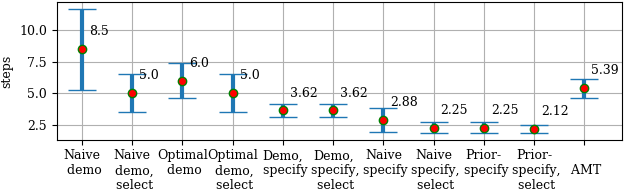
\includegraphics[width=\linewidth]{figures/avgSteps-8-AMT}
	\caption{Average number of steps required for 8 arrangement tasks chosen for the user study, by teaching strategy and human performance (AMT).}
	\label{fig:avgSteps-AMT}
\end{figure}

\begin{figure}[h]
	\centering
	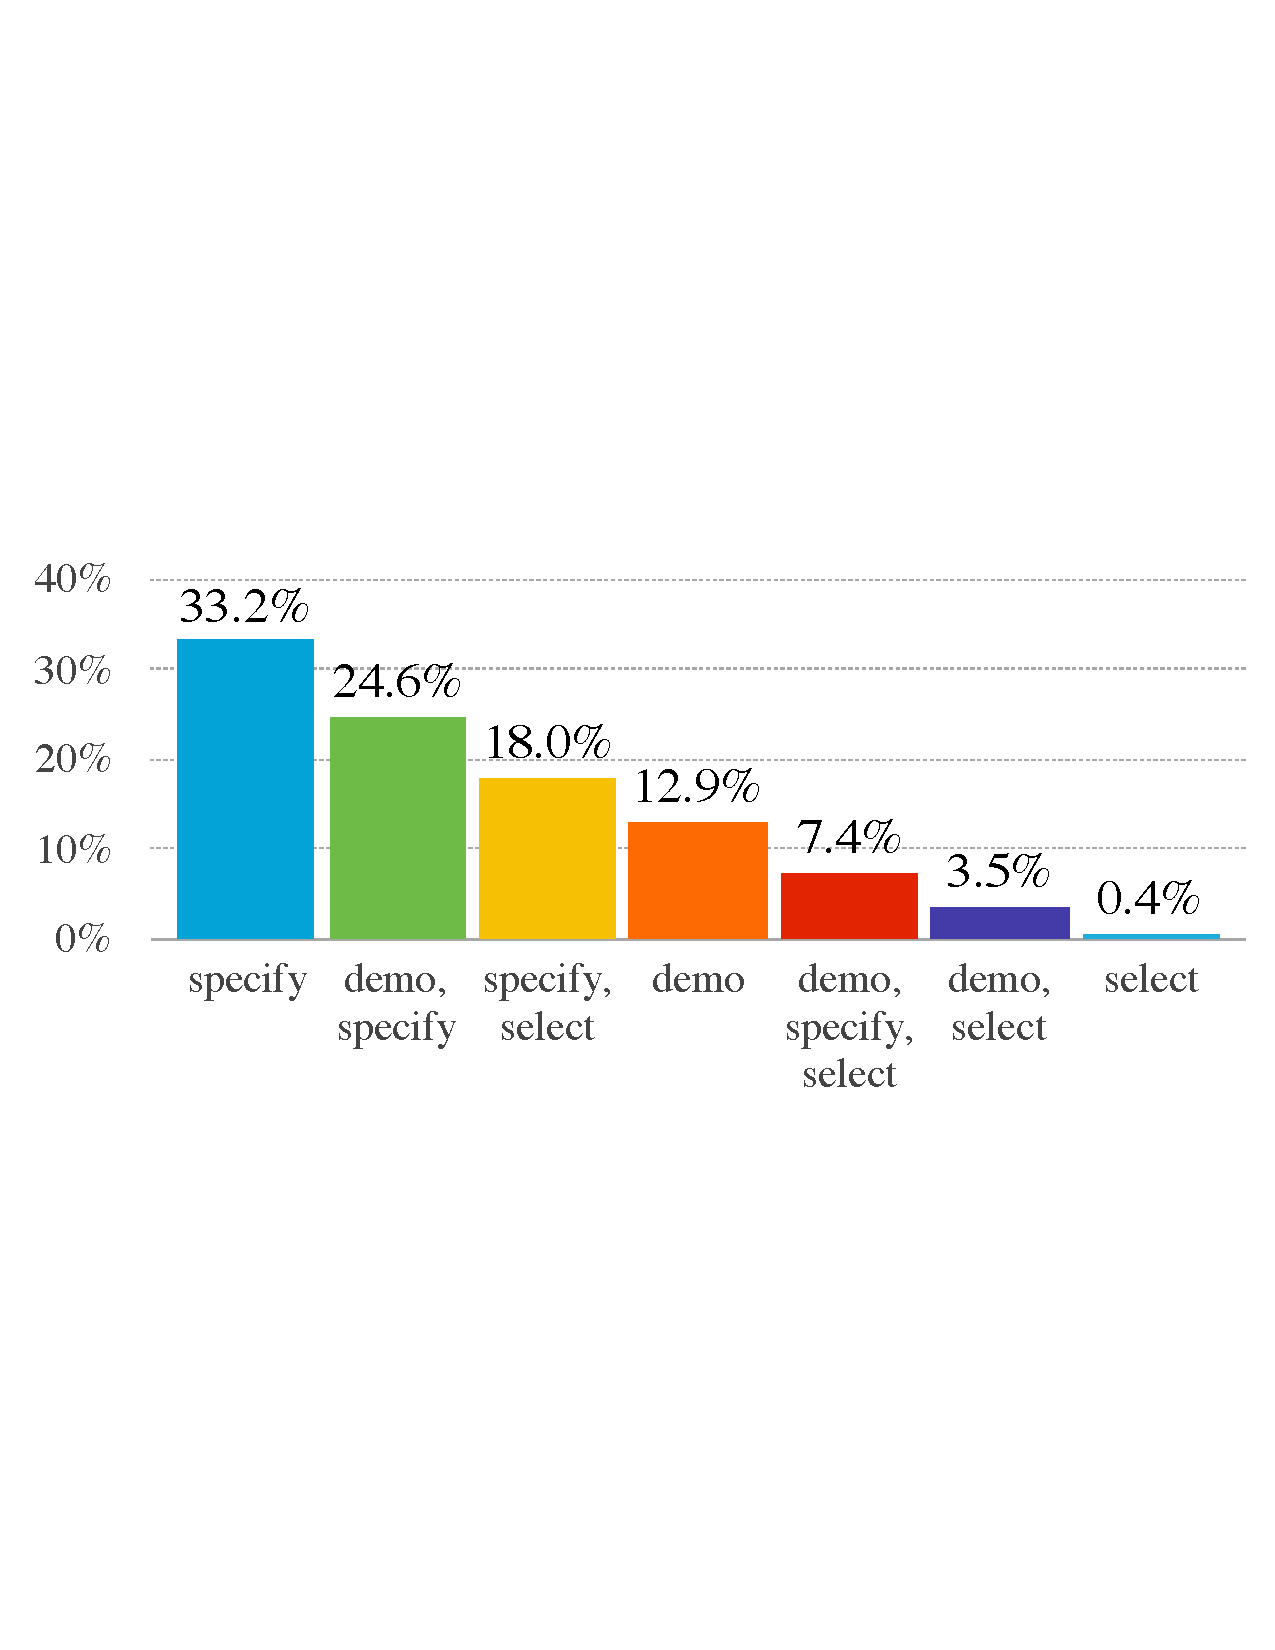
\includegraphics[width=0.7\linewidth]{figures/strategies}
	\caption{Distribution of user strategies employed in the AMT study}
	\label{fig:strategies}
\end{figure}

\begin{figure}[ht]
	\centering
	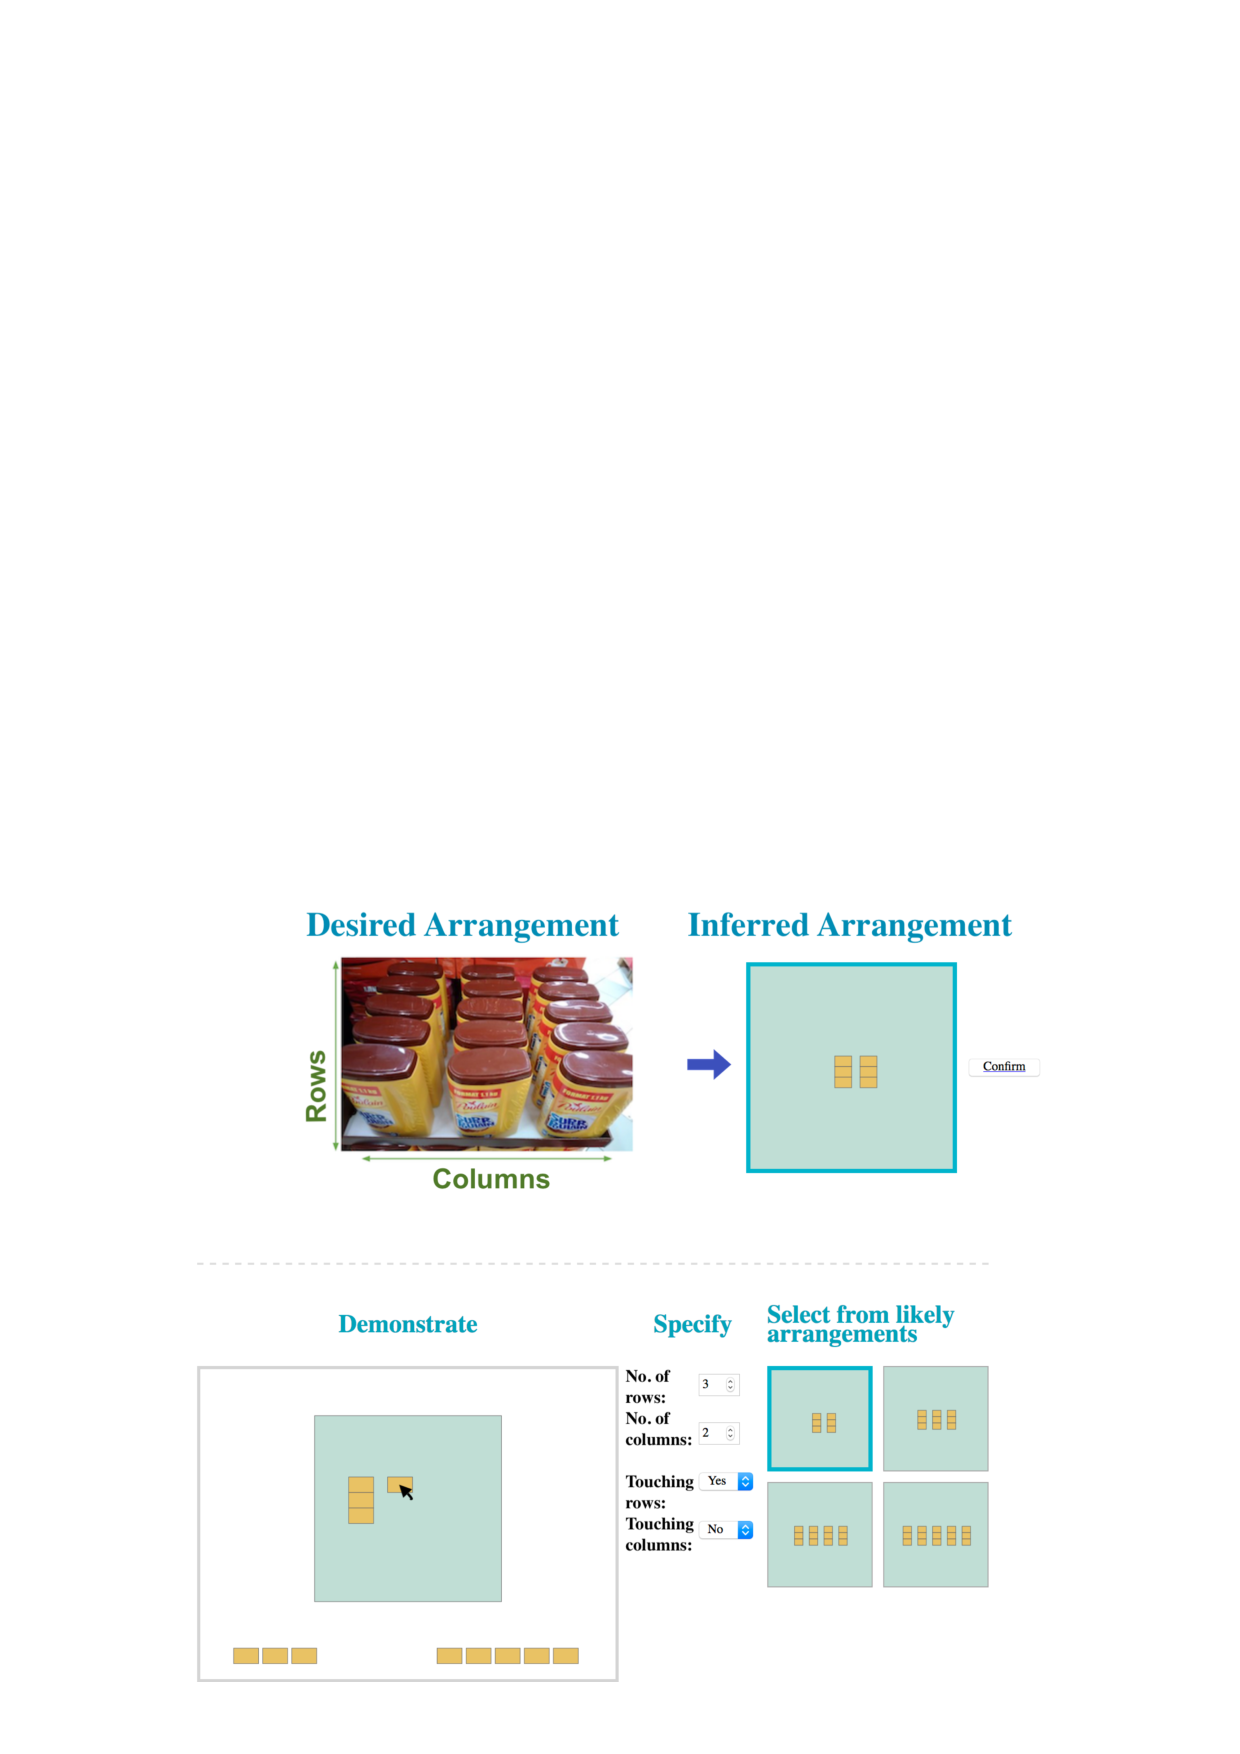
\includegraphics[width=0.9\linewidth]{figures/amt-gui}
	\caption{Simplified user-interface created to evaluate our goal inference model in an online user study. The top part shows the desired configuration with a picture and the visualisation of the current shelf arrangement inference. The bottom part has three parts corresponding to three types of programming actions the user can take: demonstration (drag-and-drop items onto shelf), specification (select parameter values from drop-down menus), and selection (choose one of the top four most likely arrangements by clicking on it).}
	\label{fig:amt-gui}
\end{figure}


%%%%%%%%%%%%%%%%%%%%%%%%%%%%%%%%%%%%%%%%%%%%%%%%%%%%%%%%%%%%%%%%%%%%%%%%%%%%%%%%
\section{System Evaluation}\label{sec:irossystemeval}

To demonstrate our full system's ability to learn and execute shelf arrangement tasks, we defined a list of benchmark tasks described in \tbl{table:tasklist}. 
The tasks varied in product type and grid configuration parameters, some of which required different manipulation actions (\eg to place an objects in touching configurations while avoiding collisions of the gripper with other objects).
We also included more complex arrangements such as off-grid cylinders and interleaved soft packaging (\fig{fig:off-grid}b,c) which were excluded from our goal inference analysis due to low frequency in the dataset. 
%We programmed each arrangement tasks as efficiently as possible using the teaching strategies from \sect{sec:irosstrategy} and reusing previously taught actions. 

\subsection{Protocol}
All tasks were programmed by one of the authors, with a subset programmed by another author to ensure consistency.
We programmed each arrangement task as efficiently as possible using the teaching strategies from Section \ref{sec:irosstrategies} and reusing previously taught actions. 
For each task, the experimenter decided what type of manipulation action was required depending on the object type and the grid configuration.
The experimenter could also decide if a new action needed to be demonstrated or if a previously existing one could be reused (as described in \sect{sec:irosimplementation}).
The actions were chosen to be as simple as possible for the given task, omitting any unnecessary gestures or movements (\eg if a simple place action was sufficient, no additional push action should be taught). When programming an action, the experimenter could let the robot execute the partial arrangement task for a subset of objects as part of the programming process to mitigate errors in the final task execution.

\begin{table}[h]
	\centering
	\caption{Benchmark tasks used for evaluating the full system implementation on the Fetch robot.}
	\label{table:tasklist}
	\begin{center}
		\begin{tabular}{clll}
			\# & Grid (n,m,s) & Used manipulation actions & Product \\ \hline
			1 & (4,1,1) not-touching & Pick and place & Tin cans \\
			2 & (2,2,2) not-touching & Pick and place & Tin cans \\
			3 & (1,4,1) touching & Pick, place, push left & Tin cans \\
			4 & (1,3,1) close distance & Pick, place, push left & Cereal boxes \\
			5 & (1,3,1) close distance & Pick, place, push left & Toothpaste \\
			6 & (3,3,1) off-grid & Pick, place, push left\&front & Tin cans \\
			7 & (3,3,1) off-grid & Pick, place, push left\&front& Soda cans \\
			8 & (2,3,1) interleaving & Pick and place from top & Candy bags \\ \hline
		\end{tabular}
	\end{center}
\end{table}


\subsection{Results}
We programmed four different manipulation actions to complete the eight benchmark tasks. 
Manipulation actions included pick, place (from front), place from top, push left, and push left\&front.
We were able to reuse these actions for similar tasks by modifying the required steps of the program.
Each task was executed successfully from start to end at least two times.
Figure \ref{fig:ppp-can} shows snapshots from the action executions of the benchmark tasks.
%\footnote{A video of the task executions can be found here: TO DO}
%For a new program, the authors demonstrated one manipulation action and specified the grid parameters directly on the interface.
%Similarly, the taught programs can be reused for other shelf arrangement tasks involving different configuration parameters and product types outside our benchmark list.
%However, manipulating certain product types depends on the robot's end-effectors, but can generally be taught by demonstration.
The evaluation demonstrates our system's capability to learn manipulation actions for the main product types, as well as soft packaging (\eg candy), which cover 98.7\% of the Freiburg dataset\footnote{Sample executions of shelf arrangement tasks can be seen at \url{https://youtu.be/liaSirH0CeM}}. 

\begin{figure}
	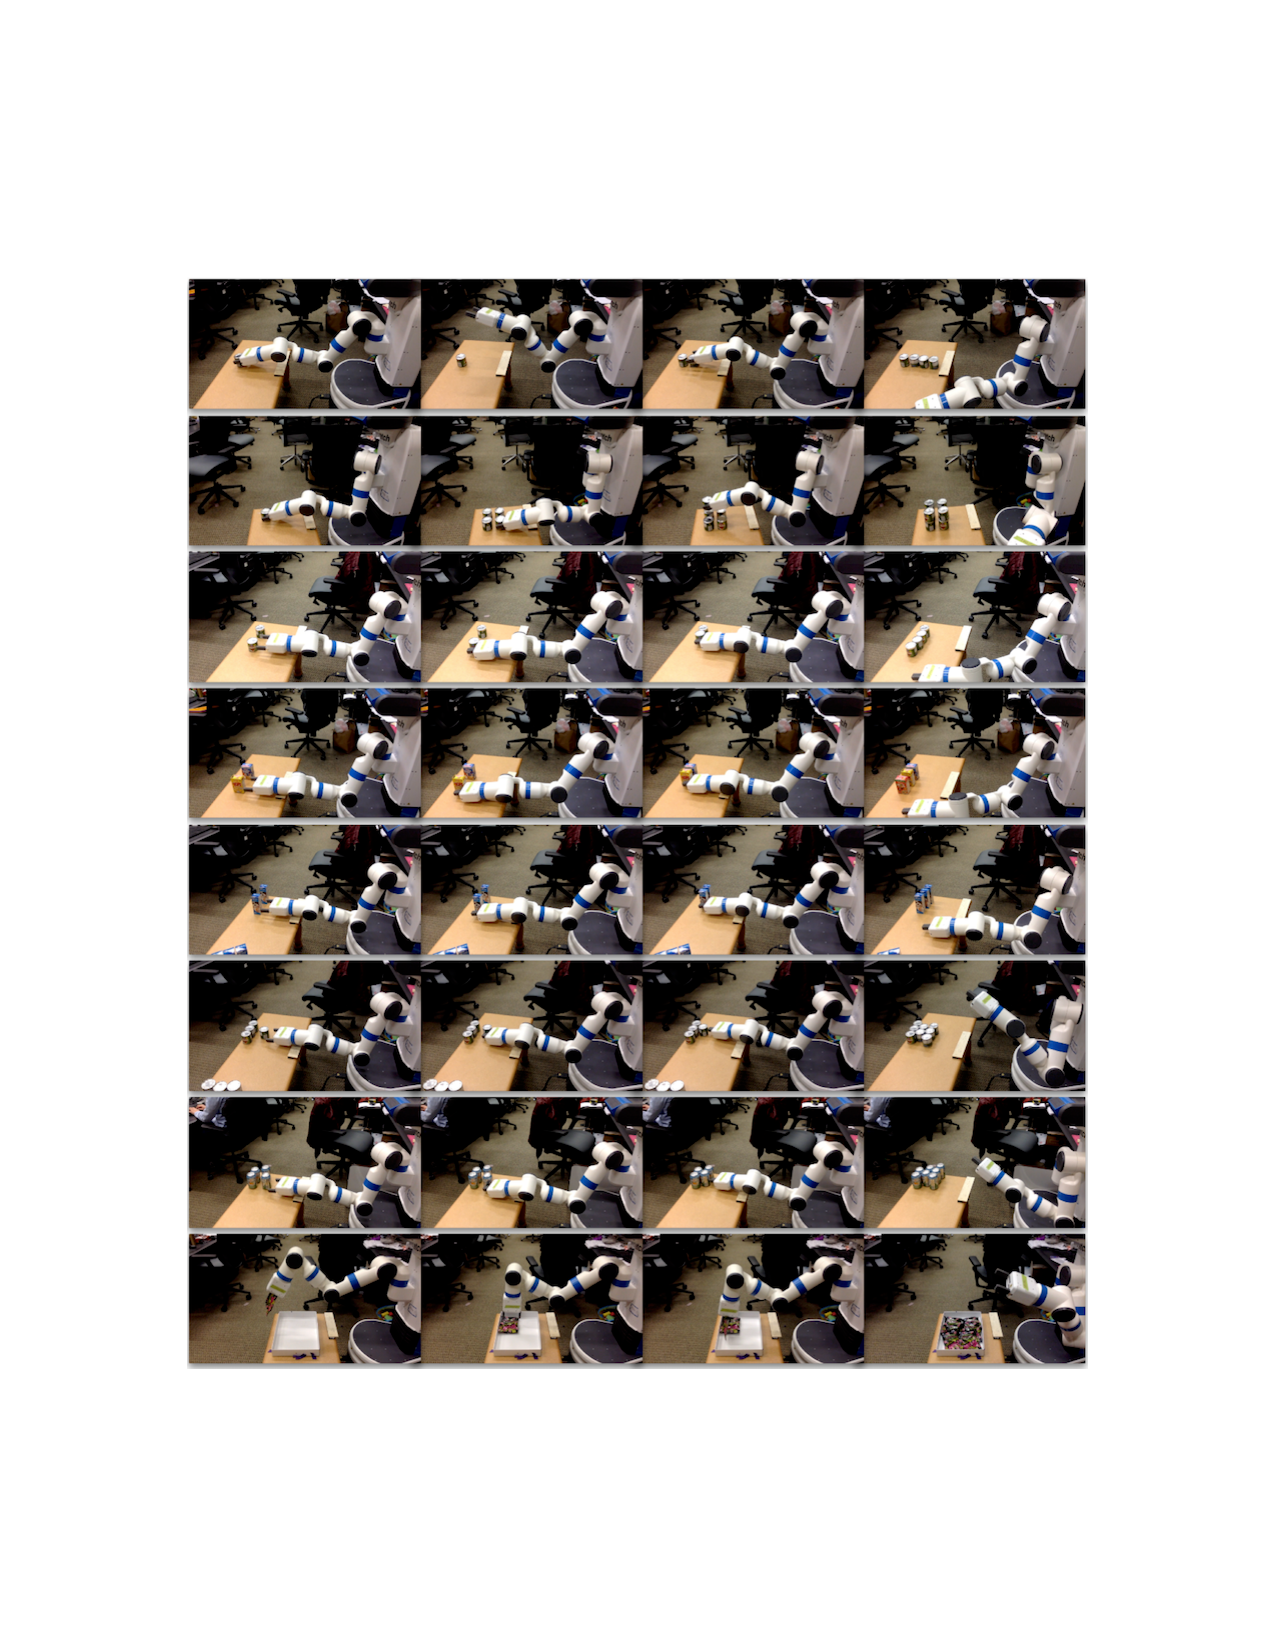
\includegraphics[width=\linewidth]{figures/frames}
	\caption{Snapshots from the executions of the eight system evaluation benchmark tasks (\tbl{table:tasklist}).}
	\label{fig:ppp-can}
\end{figure}


%%%%%%%%%%%%%%%%%%%%%%%%%%%%%%%%%%%%%%%%%%%%%%%%%%%%%%%%%%%%%%%%%%%%%%%%%%%%%%%%
\section{Discussions}\label{sec:irosdiscussions}
In the AMT study, users performed demonstrations using drag-and-drop operations which is simpler than stacking objects on a shelf with a real robot. 
As users preferred specification strategies over drag-and-drop demonstrations, it is likely that demonstrating object stacking would be less preferred as well.
Some limitations of our approach are as follows.
\begin{enumerate}
	%\item No generalisation from one item to another.
	\item Our system only considers one demonstrated manipulation action, even if multiple demonstrations are performed. An extension could consider the poses of multiple action demonstrations and infer an action adapted to a specific scenario (\eg only use push action if the gripper would collide with other landmarks).
	\item The system's perception system is limited as it does not recognise separate objects that are too close together. This limits our ability to detect demonstrated configurations for objects that are meant to be touching.
	\item We did not consider the orientation of the object (\eg product label facing front) as commonly applied in shelf organisation tasks. Our perception system only recognises the object's bounding box, so an extension could include better object recognition and object orientations.
\end{enumerate}

%%%%%%%%%%%%%%%%%%%%%%%%%%%%%%%%%%%%%%%%%%%%%%%%%%%%%%%%%%%%%%%%%%%%%%%%%%%%%%%%
\section{Conclusions}
\label{sec:irosconclusion}
In this chapter we presented an end-user robot programming system to efficiently teach a robot shelf arrangement tasks and actions.
We proposed augmenting Programming by Demonstration with domain-aware goal inference and direct user inputs to accelerate the teaching process.
Our task goal representation is based on an analysis of a large database of grocery store shelf images.
We evaluated our goal inference with different teaching strategies and with real human teachers in an online user study on AMT.
We then demonstrated our system's ability to efficiently learn and perform various shelf arrangement tasks and actions on a Fetch mobile manipulator.

In the context of this thesis, we demonstrated the generalisability of our chosen PbD approach using keyframe-based demonstration and validated its usability for end-user robot programming applications.
The main focus was to demonstrate the system's expressivity by allowing users to easily teach robots a variety of customised actions.
The implemented system is the first step towards creating the robot programming framework proposed in \chapt{chap:Contribution} and includes both teaching the robot low-level actions and a graphical interface to facilitate the end-user programming process.
The main focus for the remaining thesis is the complete implementation of the proposed framework and augmenting the graphical interface to allow intuitive navigation of the different functionalities. 
Building on top of this system, the remaining steps to implement are learning high-level action representations and integrating the task planner resulting in an end-to-end robot programming system.